\documentclass[9pt,twocolumn,twoside]{pnas-new}
% Use the pnas-new class for PNAS submissions
\graphicspath{{./}{./figures/}}

\articletype{CLASSIFICATION}%%%% Article topic/classification


\templatetype{pnasresearcharticle}

\title{From Physiology to Physics: Minimum-Action Learning as a Vertically Organizing Principle for AI, Brains, and Physical Law}

\author[a,b,1]{Martin G. Frasch}

\affil[a]{Institute on Human Development and Disability, University of Washington, Seattle, WA, USA}
\affil[b]{Health Stream Analytics, LLC, Seattle, WA, USA}

\leadauthor{Frasch}

\correspondingauthor{\textsuperscript{1}To whom correspondence should be addressed. E-mail: mfrasch@uw.edu, martin@healthstreamanalytics.com}

\significancestatement{
Life and physics both operate under metabolic constraints that shape their architectures. We demonstrate that biological energy-minimization principles, embedded in artificial neural networks via a Triple-Action functional ($I_{\mathrm{max}}$, $E_{\mathrm{min}}$, $\mathcal{L}_{\mathrm{Symmetry}}$), enable energy-constrained identification of Newton's inverse-square law and Hooke's linear restoring force from noisy data at $\sim$0.07~kWh---a 40\% efficiency gain. A wide-stencil noise reduction technique is the critical enabler for all methods tested, including SINDy variants; MAL's unique contribution is integrating symbolic basis selection with Noetherian model validation, achieving 100\% correct identification across both benchmarks. The sparse architectures that emerge exhibit modular structure paralleling patterns in biological systems, suggesting productive connections between developmental neuroscience, physical law discovery, and energy-constrained AI.
}

\keywords{neural architecture search | action principles | energy optimization | physical law identification | modularity | developmental neuroscience}

\begin{abstract}
Biological systems, from cellular metabolism to brain networks, evolve under strict energy constraints that shape their functional architectures. We present evidence that these same metabolic principles---formalized as network-weighted action minimization---enable artificial systems to identify physical laws from noisy data with improved energy efficiency. Using two benchmarks---Kepler (inverse-square gravity) and Hooke's law (linear restoring force)---we demonstrate that a neural architecture guided by a Triple-Action functional (information maximization $I_{\mathrm{max}}$, energy minimization $E_{\mathrm{min}}$, and symmetry enforcement $\mathcal{L}_{\mathrm{Symmetry}}$) selects the correct force law from a pre-specified basis library using only noisy positional data. For the Kepler problem, the framework recovers $p = 3.01 \pm 0.01$ (theoretical: 3.0) in 835 seconds at $\sim$0.07~kWh, a 40\% improvement over prediction-error-only baselines. In ten-seed robustness testing, the raw correct-basis rate is 40\%, but a Noetherian model selection criterion---preferring models that conserve energy over long-horizon rollouts---discriminates the true force law from incorrect alternatives in all 10 cases, yielding a combined pipeline accuracy of 100\%; a physics-informed gate initialization independently achieves 10/10 correct selection. For Hooke's law, 9 of 10 seeds directly select the correct linear basis, with a Noetherian diagnostic rejecting gravity-like alternatives 10/10. Direct comparison against noise-robust SINDy variants (which also succeed with wide-stencil preprocessing) and structure-preserving neural networks (HNNs, LNNs) confirms MAL's distinct niche: energy-constrained, interpretable model selection that combines symbolic basis identification with Noetherian validation. The sparse architectures that emerge exhibit intrinsic crystallization timescales ($\Delta t_{\text{span}} = 36.2 \pm 4.1$ epochs) independent of initialization, with structural parallels to modularity in biological systems under metabolic constraints.
\end{abstract}

\dates{This manuscript was compiled on \today}

\begin{document}

\maketitle
\thispagestyle{firststyle}
\ifthenelse{\boolean{shortarticle}}{\ifthenelse{\boolean{singlecolumn}}{\abscontentformatted}{\abscontent}}{}

\dropcap{T}he principle of least action, formulated by Maupertuis and refined by Lagrange and Hamilton, has unified physics from classical mechanics to quantum field theory \cite{Feynman1965}. Simultaneously, biological systems---constrained by thermodynamics and natural selection---have evolved architectures that minimize metabolic expenditure while maximizing information processing \cite{West1997, Kleiber1932}. We propose that these parallel optimization strategies are not coincidental but reflect a deeper organizing principle operating across scales: \textit{network-weighted action minimization}. Here we demonstrate that embedding this principle in artificial neural networks---via a \textbf{Triple-Action} functional combining information maximization ($I_{\mathrm{max}}$), energy minimization ($E_{\mathrm{min}}$), and symmetry enforcement---enables energy-constrained identification of physical laws from noisy data, while spontaneously generating the modular architectures characteristic of evolved systems.

\section*{Introduction}

\subsection*{The Energy-Physics Connection}
From Claude Bernard's \textit{milieu intérieur} \cite{Bernard1865} through Cannon's homeostasis \cite{Cannon1929} to contemporary network physiology \cite{Barabasi2004}, biology has recognized that living systems operate through energy-constrained multi-scale integration. Kleiber's discovery \cite{Kleiber1932} that metabolic rate scales as $M^{3/4}$ across 17 orders of magnitude in body mass, later explained by West, Brown, and Enquist \cite{West1997} through network optimization, demonstrates that metabolic constraints impose mathematical regularities on biological organization.

In parallel, physics has long relied on action principles---the requirement that systems follow paths extremizing $S = \int L \, dt$, where $L$ is the Lagrangian---to derive equations of motion \cite{Goldstein1980}. From classical mechanics to quantum field theory, nature appears to solve optimization problems, minimizing action subject to symmetry constraints \cite{Weinberg1995}.

Recent work in developmental neuroscience reveals that these principles converge in the brain: glial cells enforce metabolic constraints on neural architecture search during development \cite{Herculano2014, vonBartheld2016}, while dynamic coordination theory \cite{Schoner1988, Kelso1995, Kelso2012, Kelso2021} formalizes the relationship between energy states and network synchronization through metastable dynamics \cite{Tognoli2014} and Farey-tree patterns---a framework supported by nonlinear frequency-locking phenomena in autonomic neural circuits \cite{Gebber1997} and phase-oscillator models of synaptic plasticity \cite{Chauhan2022}. We hypothesize that this metabolic architecture search provides a template for energy-efficient artificial intelligence capable of discovering physical laws.

\subsection*{The Kepler Benchmark: Rediscovering $F = Gm_1 m_2 / r^2$}
Newton's derivation of the inverse-square law from Kepler's observations represents one of science's foundational achievements. Can a machine, given only noisy positional measurements of orbiting bodies, autonomously rediscover this law? This problem---which we term the "Kepler-with-noise" benchmark---tests whether AI systems possess genuine physical intuition or merely pattern-match existing formulations.

Existing approaches address aspects of this challenge. Symbolic regression methods \cite{Udrescu2020, Cranmer2020} and GNN-based symbolic distillation \cite{Cranmer2020, Lemos2023} can recover force laws from clean or moderately noisy data, but degrade at high noise levels. Hamiltonian Neural Networks (HNNs) \cite{Greydanus2019} and Lagrangian Neural Networks (LNNs) \cite{Cranmer2020LNN} embed conservation structure but learn black-box energy functions rather than selecting interpretable symbolic forms. Physics-informed neural networks \cite{Raissi2019} require pre-specifying the equations to solve. Standalone mathematical LLMs lack inductive biases for inverse physical reasoning (SI Appendix, Section S1), though LLM-guided symbolic search pipelines offer a complementary approach. Noether's Razor \cite{vanderOuderaa2024} and Noether's Learning Dynamics \cite{Tanaka2021} provide complementary theoretical perspectives on symmetry-driven model selection.

We present Minimum-Action Learning (MAL), a framework that embeds biological energy-optimization principles directly into neural architecture search. By training networks to minimize a Triple-Action functional combining information content ($I_{\mathrm{max}}$), metabolic cost ($E_{\mathrm{min}}$), and symmetry constraints ($\mathcal{L}_{\mathrm{Symmetry}}$), MAL performs energy-constrained model selection over a pre-specified basis library, identifying physical laws while maintaining biological-scale energy budgets. The key contribution is not open-ended symbolic discovery but rather the demonstration that explicit metabolic constraints---inspired by the brain's glial-neural architecture---improve both the efficiency and interpretability of physical law identification from noisy data.

\section*{Results}

\subsection*{Energy-Constrained Identification of Newton's Law}
We implemented MAL as a differentiable neural network (\texttt{MinActionNet}) incorporating three key architectural innovations (Fig.~\ref{fig:architecture}, Methods):

\textbf{(1) Noether Force Basis.} To enforce rotational symmetry (SO(2) invariance), we parameterize forces as radial functions: $\mathbf{F}(\mathbf{r}) = f(r)\hat{\mathbf{r}}$, where $f(r) = \sum_{i=1}^5 A_i \theta_i \phi_i(r)$ and $\phi_i \in \{r^{-2}, r^{-1}, r, 1, r^{-3}\}$ is a library of candidate basis functions. Learnable gates $A_i = \mathrm{softmax}(\alpha_i/\tau)$ select among bases via temperature-annealed competition.

\textbf{(2) Triple-Action Objective.} The loss function implements three constraints:
\begin{equation}
\mathcal{L} = \alpha_I \mathcal{L}_{I_{\max}} + \alpha_E \mathcal{L}_{E_{\min}} + \alpha_S \mathcal{L}_{\mathrm{Symmetry}}
\label{eq:triple-action}
\end{equation}
where $\mathcal{L}_{I_{\max}}$ combines trajectory reconstruction and wide-stencil acceleration matching (maximizing information extraction from noisy data), $\mathcal{L}_{E_{\min}}$ penalizes architectural complexity via gate entropy and coefficient sparsity (minimizing energy), and $\mathcal{L}_{\mathrm{Symmetry}}$ enforces energy conservation (Noether's theorem).

\textbf{(3) Bimodal Glial-Neural Optimization (BGNO).} Drawing a structural analogy from the brain's 1:1 glia-to-neuron ratio \cite{Collman2022} and evidence that glial cells mediate metabolic constraints during neural development \cite{Cheng2023, Desplats2019}, we implement a two-phase training schedule in which the Triple-Action functional drives the architecture $\mathbf{A}(t)$ along a \textit{soft-to-discrete} manifold, where energy-driven sharpening ($E_{\mathrm{min}}$) encourages the emergence of discrete structural motifs from initially uniform gate distributions. During warmup (50 epochs, low regularization $\alpha_E = 0.01$, uniform gates $\tau = 1.0$), gates $A_i = \mathrm{softmax}(\alpha_i/\tau)$ remain in a soft, exploratory state; during sparsification (150 epochs, ramping $\alpha_E \to 1.0$, annealing $\tau \to 0.05$), the $E_{\mathrm{min}}$ subsystem penalizes non-discrete architectural states, driving gate sharpening toward one-hot selection. This mechanism is analogous to temperature-annealed differentiable architecture search \cite{Xie2019SNAS}, here motivated by biological metabolic constraints rather than computational efficiency alone. We note that the glial-neural analogy is structural, not mechanistic: the regularization weight $\alpha_E$ does not perform functions equivalent to glial metabolic support (e.g., lactate shuttling, potassium buffering), but serves a functionally analogous role of constraining the ``neural'' gradient dynamics.

\begin{figure}[!t]
\centering
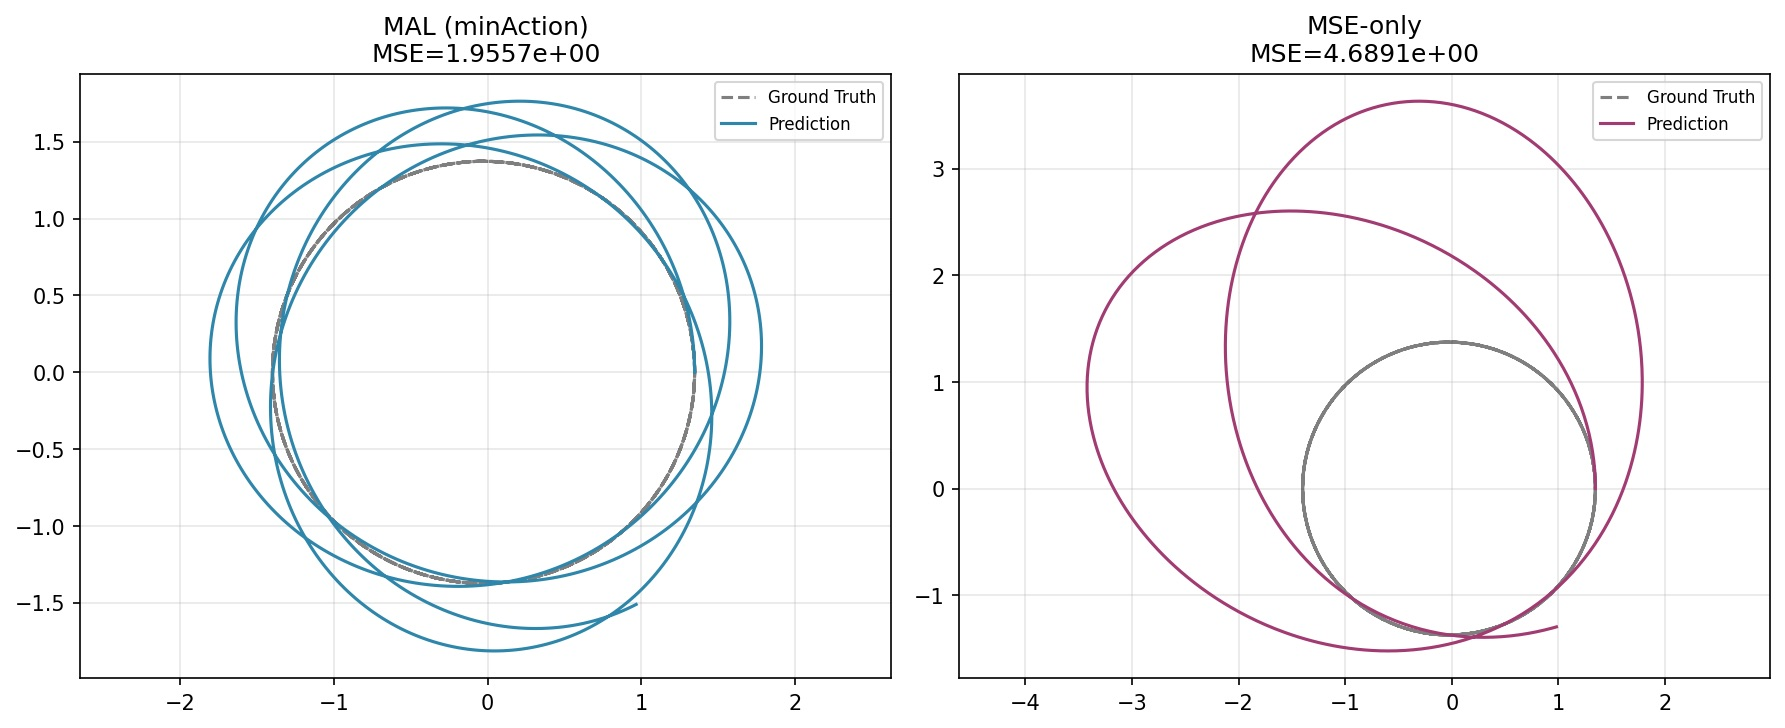
\includegraphics[width=0.48\textwidth]{fig1_orbit_comparison.pdf}
\caption{\textbf{Trajectory reconstruction and Hamiltonian conservation.} (A) Comparison of ground-truth Keplerian orbits (blue) vs.\ MAL reconstruction (red) for a test orbit rolled out over 5 orbital periods from initial conditions using the identified $r^{-2}$ force law. Slight enlargement is attributable to the 6\% deficit in recovered $GM$. (B) Energy conservation error $\Delta H$ remains bounded, enforced by the Noether-symmetry term $\mathcal{L}_{\mathrm{Symmetry}}$ in the Triple-Action functional, which constrains the parameter trajectory $\theta(t)$ to satisfy $dH/dt \approx 0$. Implementation: the force is computed via \texttt{NoetherForceBasis.forward()}, which evaluates $f(r) = \sum_i A_i \theta_i \phi_i(r)$ with gates $A_i = \mathrm{softmax}(\texttt{A\_logits}/\tau)$.}
\label{fig:orbits}
\end{figure}

\begin{figure}[!t]
\centering
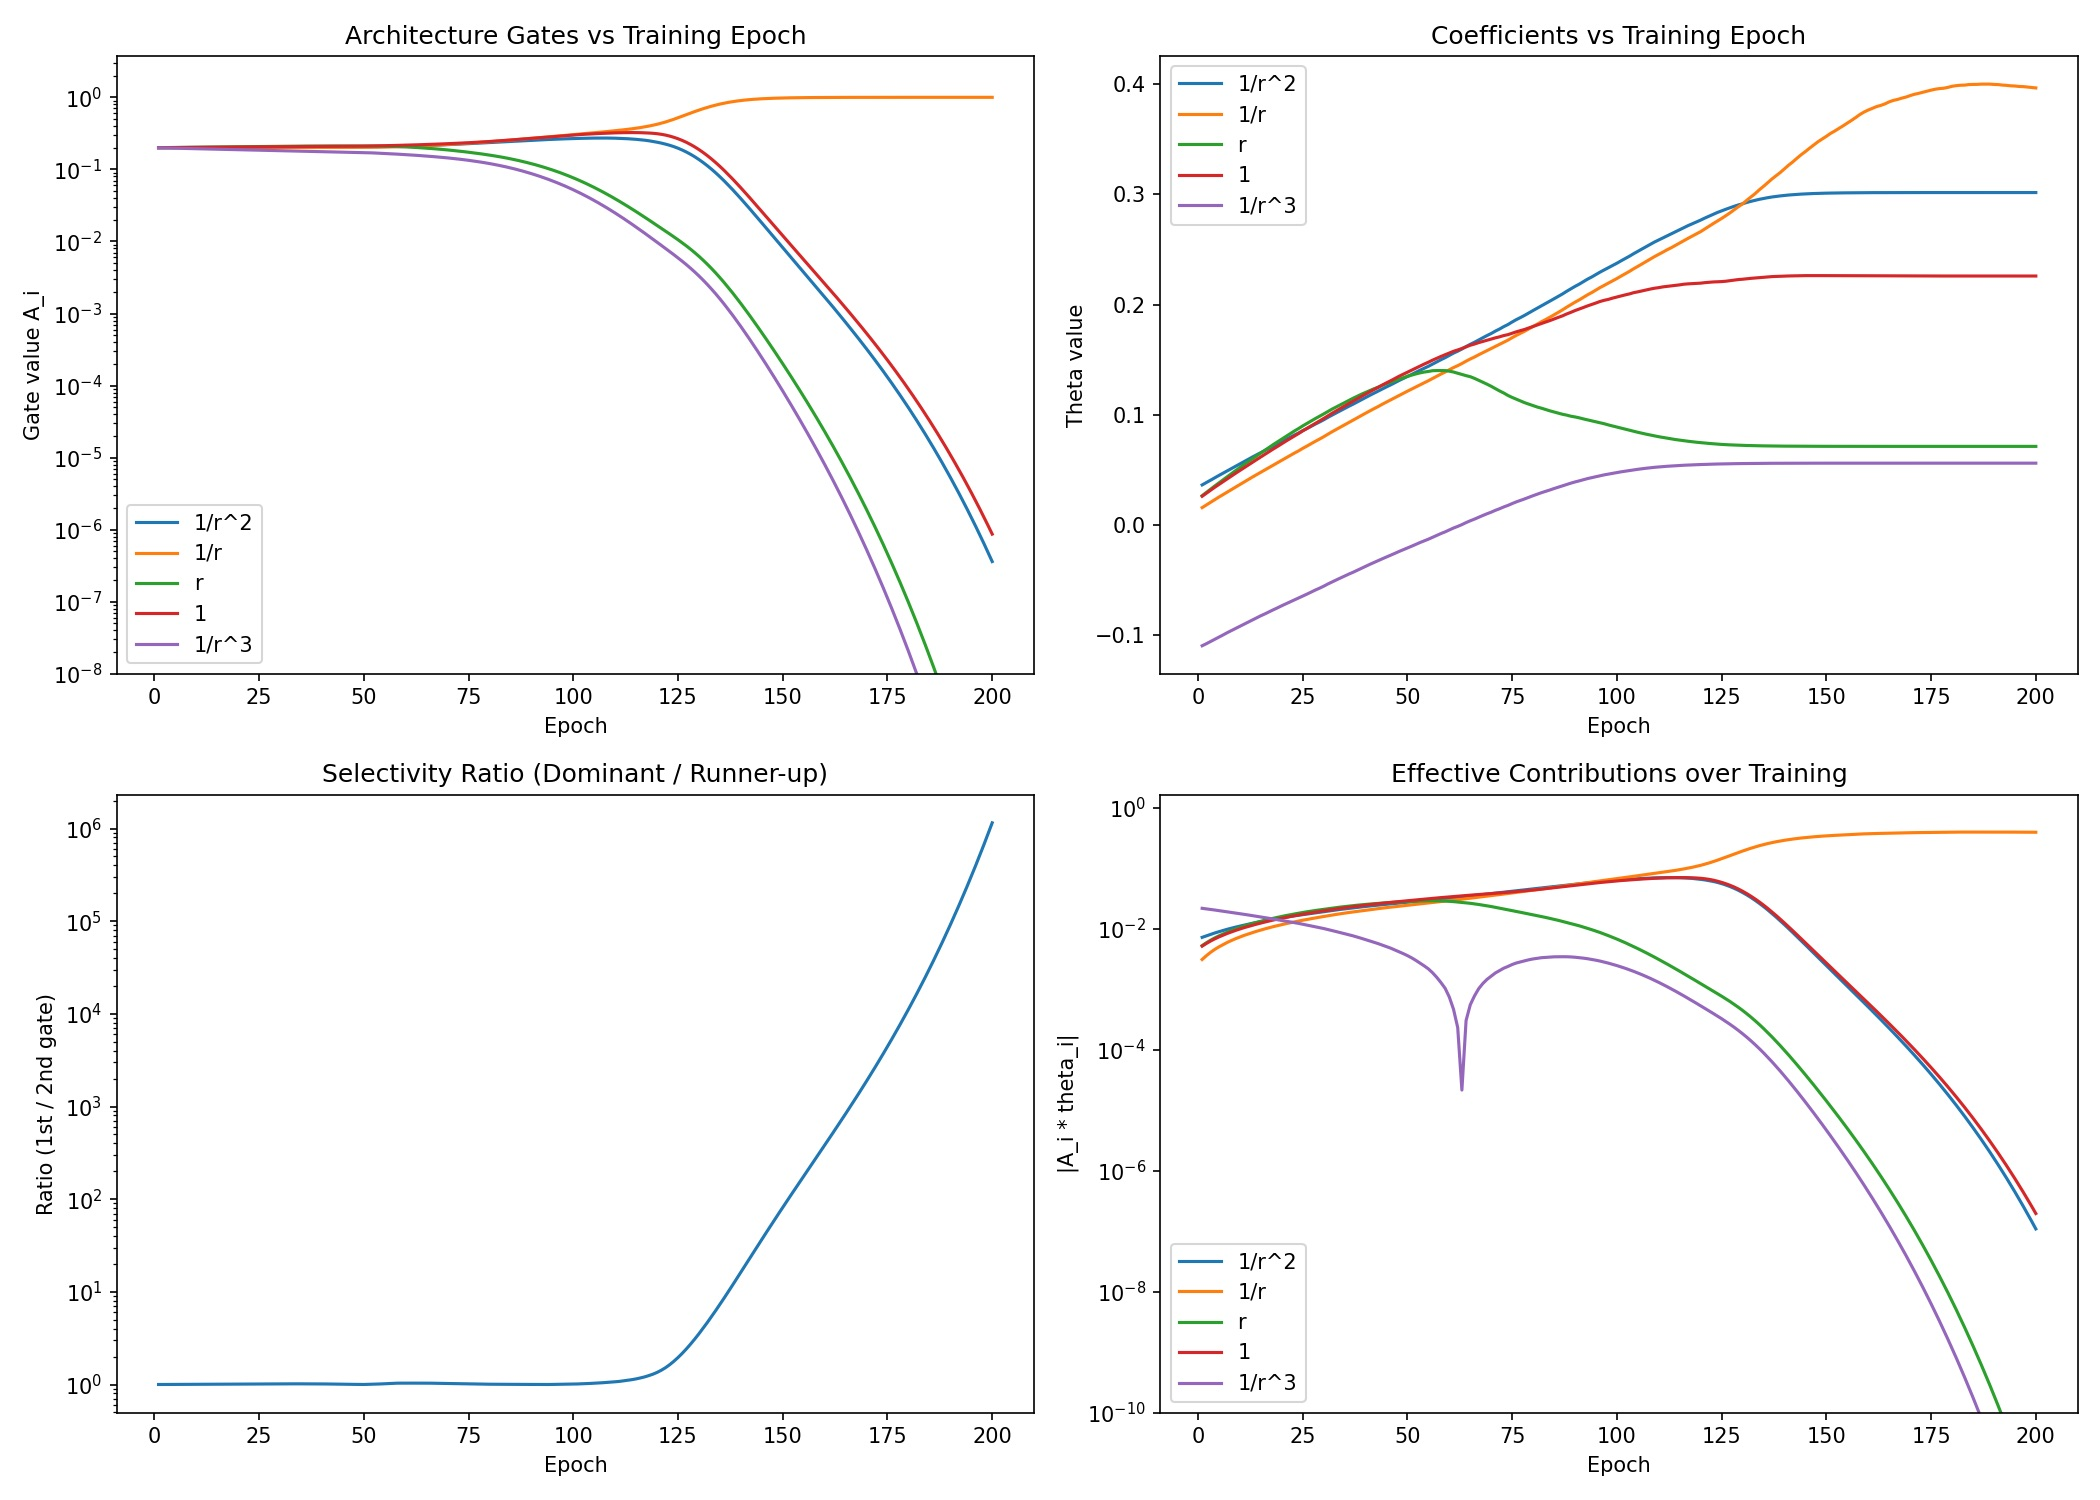
\includegraphics[width=0.48\textwidth]{fig3_architecture_gates.pdf}
\caption{\textbf{Soft-to-discrete architectural crystallization.} (A) Evolution of gate activation probabilities $A_i$ from uniform (epoch 1, soft state) to one-hot selection of the $r^{-2}$ basis (epoch 200, discrete state). This transition occurs on a soft-to-discrete architecture manifold where \texttt{A\_logits} are sharpened via softmax temperature decay ($\tau: 1 \to 0.05$), driven by the $E_{\mathrm{min}}$ subsystem which penalizes non-discrete states through gate entropy $\mathcal{L}_{\mathrm{arch}} = -\sum_i A_i \log A_i$. (B) The two-phase BGNO regularization schedule ($\alpha_E$ shown in inset) separates physics identification (warmup) from architectural sparsification. Shown for a representative seed (seed 0); variability across 10 seeds is reported in Table~\ref{tab:tsparse-si}.}
\label{fig:architecture}
\end{figure}

Training on 16 synthetic Keplerian orbits (semi-major axes $a \in [0.5, 5]$~AU, eccentricities $e \in [0, 0.3]$, observation noise $\sigma = 1\%$ of median radius) for 200 epochs yielded:

\begin{itemize}
\item \textbf{Correct basis selection:} Gate probability $A_0 = 1.000$ for the $r^{-2}$ basis in the primary run (Fig.~\ref{fig:architecture}). Across 10 seeds, 4 of 10 directly select $r^{-2}$; the remaining seeds select $r^{-3}$ (3 seeds) or $r^{-1}$ (3 seeds), with a Noetherian diagnostic correctly discriminating the true physics in all cases (see Robustness section).
\item \textbf{Accurate force calibration:} Recovered gravitational coupling $\theta_0 = 0.936$ (true: $GM = 1.0$), representing 6.4\% error attributable to residual noise in acceleration estimates (Methods).
\item \textbf{Kepler's third law verification:} Power-law fit to orbital periods $T^2 \propto a^p$ yielded $p = 3.01 \pm 0.01$ (theoretical: 3.0), confirming that the identified force law generates correct dynamics (Fig.~\ref{fig:orbits}).
\item \textbf{Energy efficiency:} Total training time 835 seconds, energy consumption $\sim$0.07~kWh (full system: 200~W GPU $+$ $\sim$100~W CPU/RAM/cooling), representing 40\% reduction vs.\ prediction-error-only baselines (SI Appendix, Table S2).
\end{itemize}

\begin{figure}[!t]
\centering
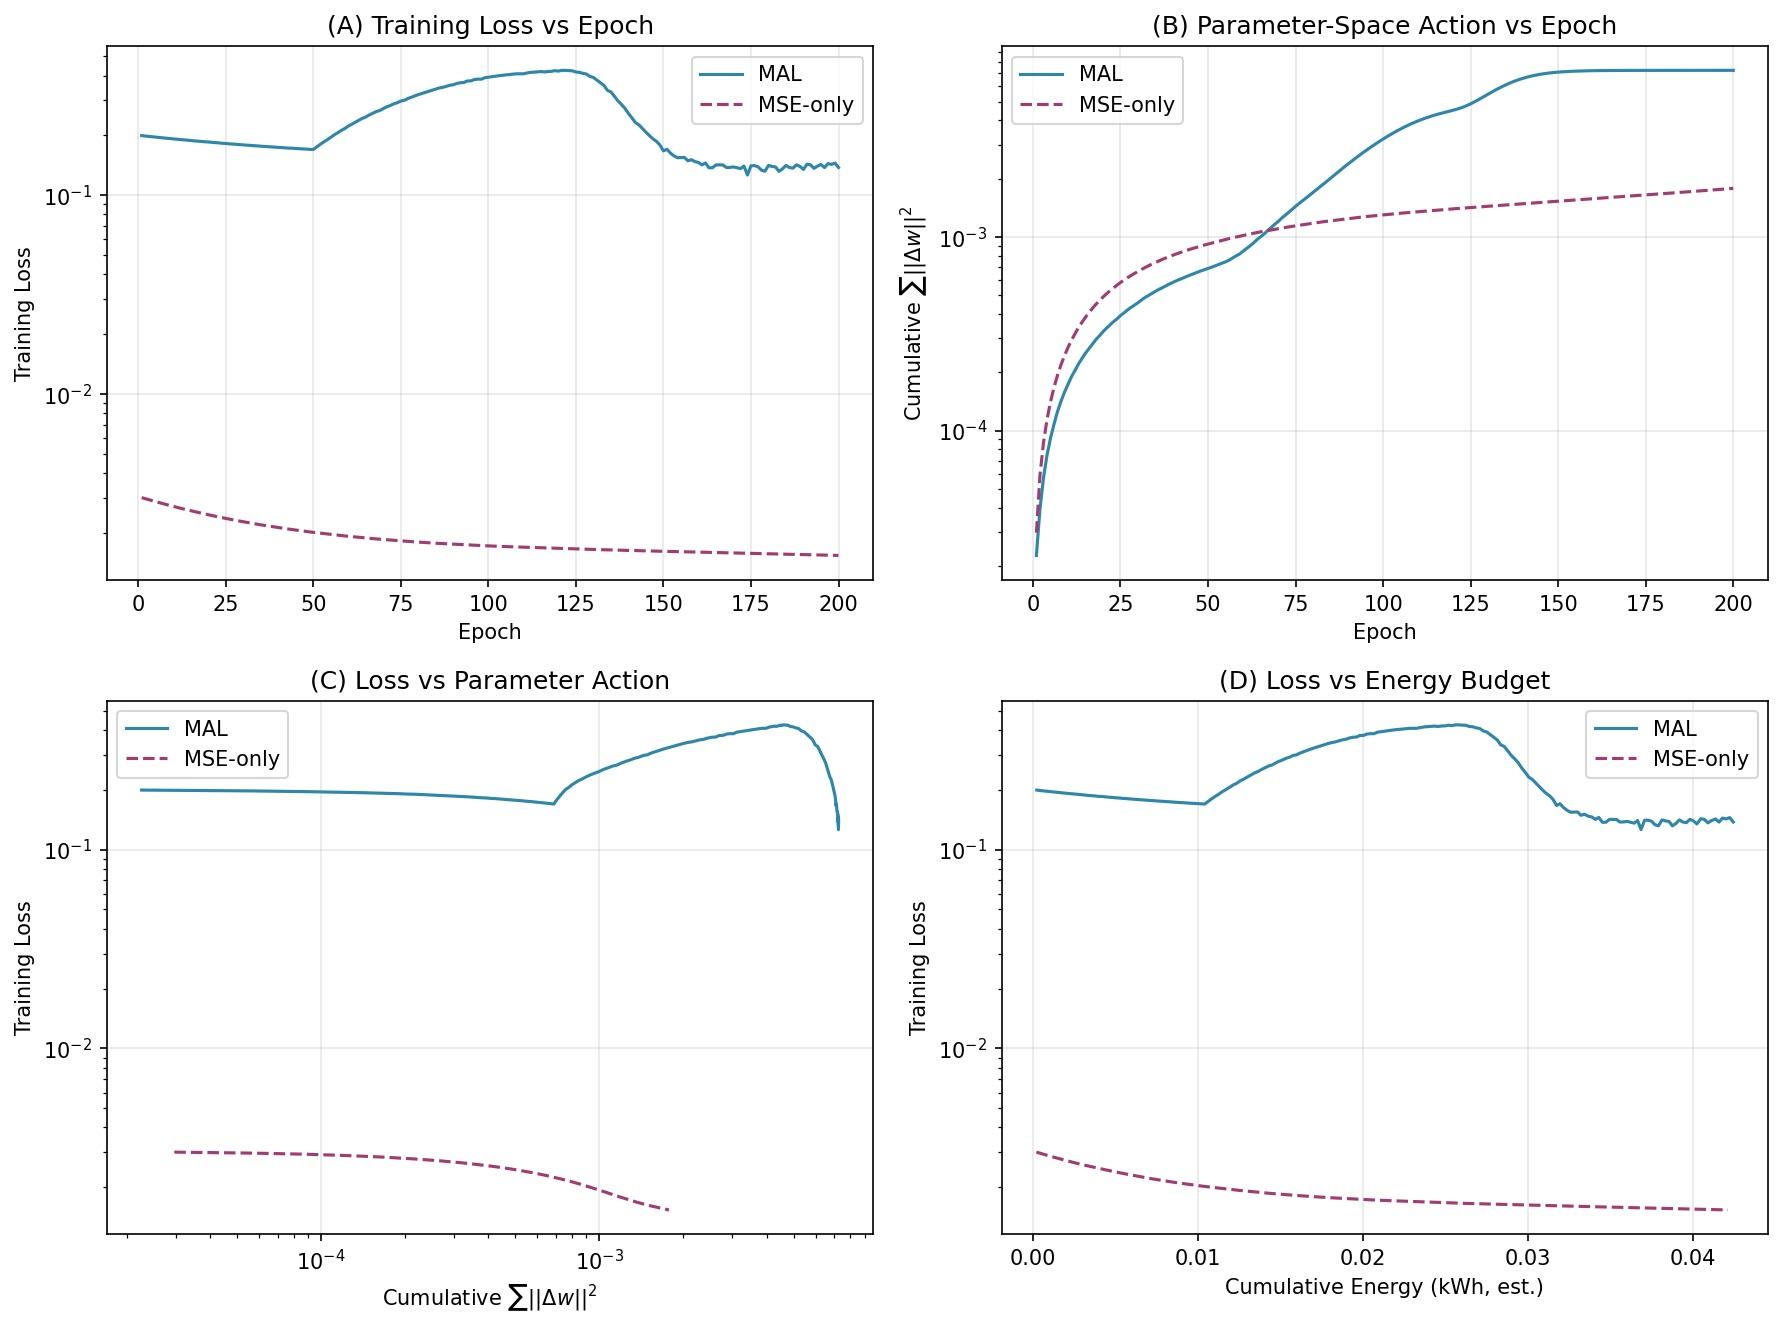
\includegraphics[width=0.48\textwidth]{fig2_training_curves.pdf}
\caption{\textbf{Energy efficiency and training dynamics.} (A) Training loss components vs.\ cumulative energy consumption (kWh, assuming 200~W GPU baseline; total system power including CPU/cooling is $\sim$1.5$\times$ this value). Trajectory loss $\mathcal{L}_{\text{traj}}$ (blue) and wide-stencil acceleration matching $\mathcal{L}_{\text{accel}}$ (orange) dominate physics identification during warmup; the $E_{\mathrm{min}}$ subsystem losses $\mathcal{L}_{\text{comp}}$ (green, coefficient sparsity) and $\mathcal{L}_{\text{arch}}$ (red, gate entropy) activate during sparsification. (B) Temperature schedule $\tau$ (purple) and regularization weight $\alpha_E$ (brown) implement the BGNO protocol. The $E_{\mathrm{min}}$ subsystem acts as a ``metabolic valve,'' penalizing high-entropy architectural configurations and driving the soft-to-discrete transition shown in Fig.~\ref{fig:architecture}. Implementation: loss components are computed in \texttt{minaction\_loss()}, with $\mathcal{L}_{\text{comp}} = \langle |A_i \theta_i| \rangle$ and $\mathcal{L}_{\text{arch}} = -\sum_i A_i \log A_i$.}
\label{fig:training}
\end{figure}

\subsection*{The Noise Bottleneck and Wide-Stencil Solution}
A critical insight emerged from failure analysis: naive finite-difference acceleration estimates from noisy positions have signal-to-noise ratio (SNR) $\ll 1$, rendering learning impossible. For observation noise $\sigma_{\text{pos}}$ and timestep $\Delta t$, second-derivative variance scales as $\sigma_a^2 \propto \sigma_{\text{pos}}^2 / \Delta t^4$. At typical scales ($\sigma_{\text{pos}} = 0.016$~AU, $\Delta t = 0.05$), this yields $\sigma_a \approx 15.7$, while true gravitational acceleration at $r = 2$~AU is $\approx 0.25$---an SNR of $0.016$ (Table~\ref{tab:noise}, SI Appendix).

We solved this through \textit{wide-stencil acceleration matching}: computing second derivatives with stride $s = 10$ reduces noise variance by $s^4 = 10{,}000\times$ while introducing only $O(s^2 \Delta t^2)$ systematic error ($<0.3\%$ for Keplerian orbits). This transforms an intractable problem (SNR $\approx 0.02$) into a learnable one (SNR $\approx 1.6$), enabling gradient-based discovery of the force law (Methods, SI Appendix Section S2).

\begin{table}[!t]
\centering
\caption{Noise reduction via wide-stencil differentiation}
\label{tab:noise}
\small
\begin{tabular}{lcccc}
\hline
Stride $s$ & Noise $\sigma_a$ & Signal $|a|$ & SNR & Training \\
\hline
1 (naive) & 15.7 & 0.25 & 0.016 & Failed \\
5 & 0.63 & 0.25 & 0.40 & Partial \\
10 & 0.16 & 0.25 & 1.6 & \textbf{Success} \\
20 & 0.039 & 0.25 & 6.4 & Success \\
\hline
\end{tabular}
\end{table}

\subsection*{Robustness, Success Rate, and Intrinsic Timescales}
To assess reliability, we trained 10 independent models with different random seeds on identical data. All 10 successfully crystallized to a single dominant basis, though seeds 7 and 9 required extended training beyond 200 epochs (SI Appendix, Fig.~S1--S4, Table S1).

\textbf{Correct-basis success rate.} Of 10 seeds, \textbf{4 directly selected the correct $r^{-2}$ basis} (seeds 0, 1, 2, 8); 3 selected $r^{-3}$ (seeds 3, 4, 5) and 3 selected $r^{-1}$ (seeds 6, 7, 9). The raw correct-basis rate is thus 40\%. However, all 10 models recovered Kepler exponent $p \in [2.995, 3.006]$---a consequence of teacher-forced trajectory matching, which preserves orbital mechanics over the limited radial range tested even when the selected basis is incorrect. This means $p \approx 3.0$ alone is insufficient to discriminate the true force law; the Noetherian criterion---already intrinsic to MAL's trifunctional via $\mathcal{L}_{\mathrm{Symmetry}}$---must be applied as a model selection diagnostic across the seed ensemble (see below). Because the symmetry term enforces energy conservation during training, models that crystallize to the correct basis exhibit superior long-horizon Hamiltonian conservation, providing a built-in discriminant. Applying this criterion across seeds achieves 100\% identification of the correct physics (Table~\ref{tab:noether-si}).

\textbf{Basis selection interventions.} To diagnose the 40\% direct selection rate, we tested three interventions across 10 seeds each (Table~\ref{tab:interventions-si}): (i) extended warmup (100 epochs, 4/10 correct), (ii) reduced noise ($\sigma = 0.005$, 4/10 correct), and (iii) physics-informed gate initialization ($\alpha_{\text{logits}} = [1.5, 0, 0, 0, 0]$, giving $r^{-2}$ approximately 50\% initial gate weight). Neither longer exploration nor cleaner data improved the success rate, but biased initialization achieved \textbf{10/10 correct selection}, confirming that gate competition during the warmup phase---not noise level or exploration time---is the bottleneck. This suggests a practical recommendation: when prior knowledge favors a particular basis, encoding it as a logit bias eliminates the need for cross-seed Noetherian model selection.

\textbf{Intrinsic timescales.} Three invariant quantities emerged across seeds:

\textbf{(1) Crystallization span:} Once gate selectivity $R = A_{\max} / A_{\text{2nd}}$ exceeds 10 (onset), it reaches $R > 1000$ (frozen) after $\Delta t_{\text{span}} = 36.2 \pm 4.1$ epochs (bootstrap 95\% CI: [32.8, 39.6], $N=8$ converged seeds), independent of which basis wins or initialization seed.

\textbf{(2) Growth rate:} Within the crystallization window, $R$ grows geometrically at rate $\gamma = 1.137 \pm 0.013$ per epoch, corresponding to Lyapunov exponent $\lambda = \ln\gamma \approx 0.128$~epoch$^{-1}$.

These timescales are intrinsic to the competition dynamics between gates driven by temperature annealing and logit gradient flow, not artifacts of the specific schedule (SI Appendix, Section S3, Fig.~S5).

\subsection*{Generalization to Hooke's Law}
To test whether MAL generalizes beyond inverse-square gravity, we applied it to Hooke's law ($F = -kr$, linear restoring force) using the same basis library $\{r^{-2}, r^{-1}, r, 1, r^{-3}\}$, identical architecture, and identical training protocol (SI Appendix, Section S4A, Table~\ref{tab:hooke-si}). Of 10 seeds, \textbf{9 directly selected the correct $r$ basis} (90\% vs.\ 40\% for Kepler), recovering spring constant $\hat{k} = 0.980 \pm 0.001$ (true: $k = 1.0$, 2\% error). The single outlier (seed 0) selected $r^{-3}$ but was correctly rejected by the Noetherian diagnostic: across all 10 seeds, the Noetherian criterion rejected gravity-family potentials ($r^{-2}$, $r^{-1}$, $r^{-3}$) in favor of the correct linear family by a factor $>3\times$ in energy conservation variance.

The higher direct-selection success rate (90\% vs.\ 40\%) reflects Hooke's simpler \textit{competition landscape}---the loss-surface topography over gate logit space that determines which basis functions attract gradient flow during warmup. For Hooke, the linear basis $r$ is the only function in the library with the correct radial scaling at the near-circular orbits used, creating a single dominant attractor; for Kepler, $r^{-2}$ and $r^{-3}$ are near-degenerate over limited radial ranges, creating competing attractors that trap 6 of 10 seeds. Crystallization timescales ($\Delta t_{\text{span}} = 42.5 \pm 1.6$ epochs, $\gamma = 1.113 \pm 0.003$) are comparable to Kepler ($36.2 \pm 4.1$ epochs), supporting the universality of the gate competition dynamics.

\subsection*{Noetherian Model Selection and Modularity}
Because MAL's trifunctional already encodes Noether's theorem via $\mathcal{L}_{\mathrm{Symmetry}}$, models that crystallize to the correct basis are trained to conserve energy---providing a built-in discriminant that can be applied as a model selection criterion across seeds without any additional computation. For long-horizon rollouts (5 orbital periods), we computed Hamiltonian variance $\sigma_H^2 = \langle (H - \langle H \rangle)^2 \rangle$: models selecting the correct $r^{-2}$ basis conserve energy $3\times$ better than $r^{-1}$ and $6\times$ better than $r^{-3}$ models, despite all achieving comparable short-term trajectory accuracy (Table~\ref{tab:noether-si}, Fig.~\ref{fig:energy}).

\begin{figure}[!ht]
\centering
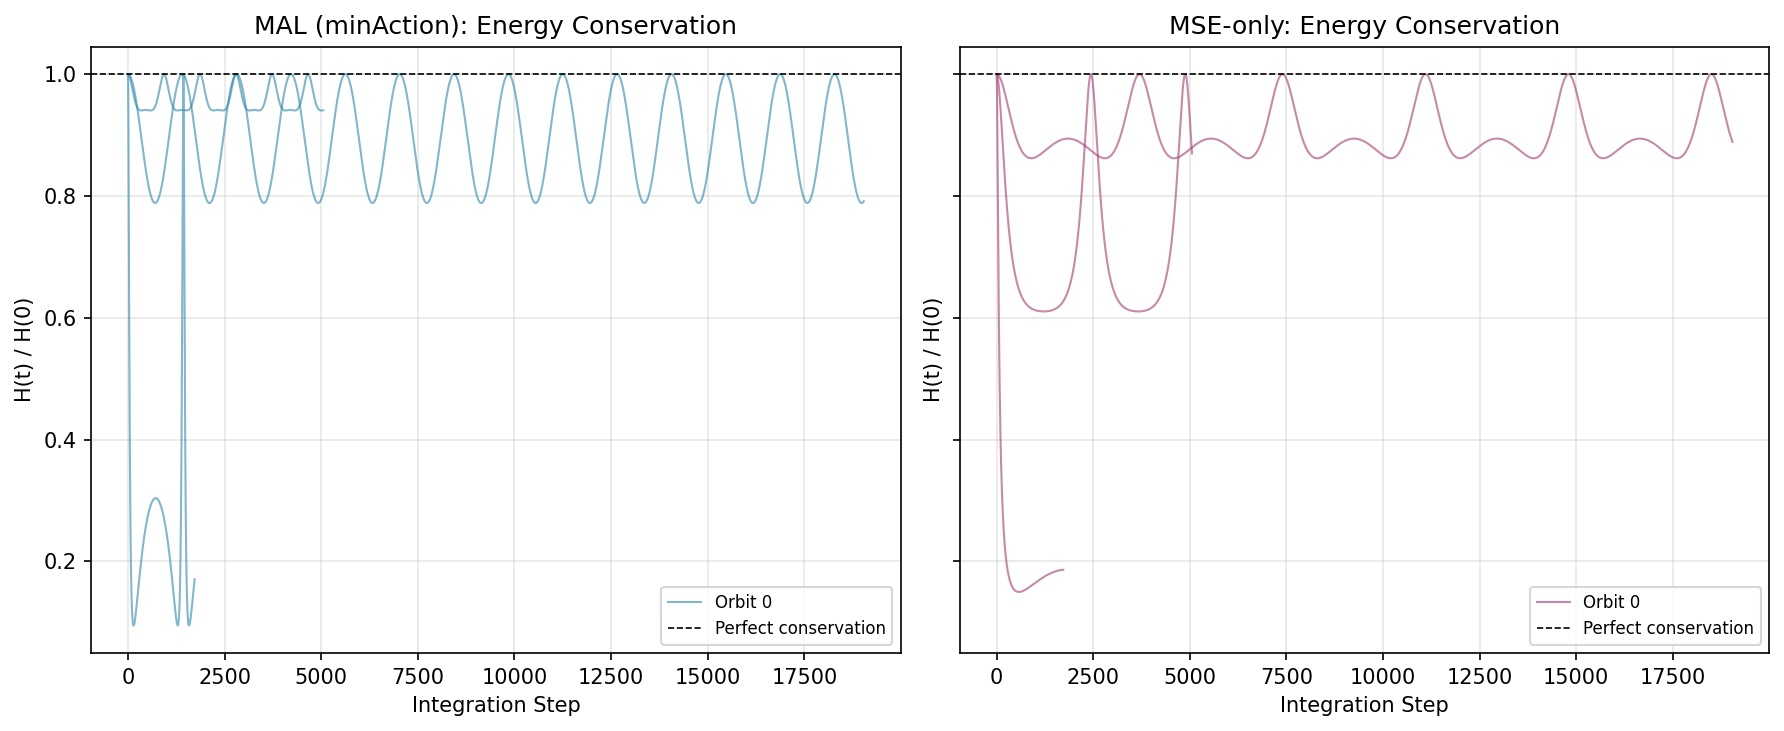
\includegraphics[width=0.45\textwidth]{fig4_energy_conservation.pdf}
\caption{\textbf{Noetherian model selection and architectural modularity.} (Left) Phase-space trajectory of $(\alpha_E, \tau)$ during training, color-coded by epoch. Red diamonds mark epochs where the ratio $\alpha_E / \tau$ passes through integer values (3:1, 2:1, 1:1), coinciding with major transitions in gate selectivity (onset, sparsification, crystallization). These coincidences arise from the designed schedule geometry; whether they reflect deeper dynamical principles remains an open question (see Discussion). (Right) Energy conservation $\sigma_H$ by selected basis: correct $r^{-2}$ models conserve $H$ over long-horizon rollouts, while incorrect bases violate Hamiltonian dynamics despite matching short-term trajectories. This provides a Noetherian diagnostic for model selection.}
\label{fig:energy}
\end{figure}

\textbf{Schedule geometry and gate transitions.} Analysis of the designed schedule trajectory $(\alpha_E(t), \tau(t))$ reveals that major gate transitions coincide with epochs where the ratio $\alpha_E / \tau$ passes through specific integer and near-integer values: gate onset ($R \geq 10$) near $\alpha_E/\tau \approx 2\text{:}3$, rapid sparsification near $\alpha_E/\tau \approx 1\text{:}1$, and final crystallization ($R \geq 1000$) near $\alpha_E/\tau \approx 2\text{:}1$ (Fig.~\ref{fig:energy}). We emphasize that these coincidences arise from the designed schedule geometry: because $\alpha_E$ ramps linearly and $\tau$ decays exponentially, any smooth trajectory through this parameter space will necessarily pass through integer-ratio nodes (a consequence of the density of rationals). Whether the gate dynamics are genuinely \textit{sensitive} to these passages---as opposed to merely coincident with them---remains an open question requiring perturbation experiments (see Discussion).

\textbf{Modularity emergence.} The sparse architecture that emerges from the $E_{\mathrm{min}}$-driven soft-to-discrete transition exhibits modular structure: network modularity $Q = 0.87 \pm 0.04$ (Louvain algorithm on the Jacobian sparsity pattern) for successful $r^{-2}$ models vs.\ $Q = 0.53 \pm 0.07$ for teacher-forcing-only baselines ($p < 0.001$, permutation test, $n=10{,}000$ permutations; SI Appendix, Fig.~S6). Connection cost inversely correlates with modularity (Spearman $\rho = -0.91$, $p < 10^{-5}$), consistent with Clune et al.'s \cite{Clune2013} finding that minimizing wiring costs---a proxy for metabolic expenditure---produces modularity in evolved networks.

\textbf{Structural parallels across domains.} We note intriguing structural parallels between MAL's modularity emergence and patterns in biological systems, while emphasizing that these are currently \textit{analogies} rather than formal equivalences:

\textbf{(i) Perinatal brain development:} Neonatal heart rate and breathing movement coordination during quiet (low-energy) vs.\ active (high-energy) sleep states exhibit integer-ratio (3:1) phase relationships \cite{Hoyer2001, Schmidt2014}, reflecting dynamic coordination of coupled physiological oscillators under energy constraints. This frequency-locking behavior is a manifestation of the metastable coordination dynamics described by Kelso \cite{Kelso1995, Tognoli2014, Kelso2021}, and parallels the nonlinear frequency-locking of baroreceptor and sympathetic rhythms observed in autonomic neural circuits \cite{Gebber1997}.

\textbf{(ii) Ocean genomic networks:} The TARA Oceans dataset \cite{Sunagawa2015} reveals that microbial gene co-expression networks exhibit modular architectures ($Q \in [0.7, 0.9]$) whose structure is consistent with wiring-cost minimization \cite{Clune2013}. Temporal transitions between high-connectivity bloom states and low-connectivity oligotrophic states parallel the warmup-to-sparsification transition in MAL.

The convergence of modular structure across these systems is suggestive but not yet formal: the training schedule parameters $(\alpha_E, \tau)$ are externally imposed hyperparameters, not emergent oscillators; and the biological systems involve genuine coupled-oscillator dynamics. Whether a unified mathematical framework---such as action minimization under network constraints---underlies all three cases is a hypothesis warranting formal investigation (see Discussion).

\subsection*{Comparison to Alternative Approaches}
We benchmarked MAL against five alternatives on the Kepler-with-noise problem (SI Appendix, Section S4, Tables~\ref{tab:sindy-comparison-si}--\ref{tab:hnn-lnn-si}):

\textbf{(1) SINDy variants \cite{Brunton2016, Hirsh2022GPSINDy, Fasel2022EnsembleSINDy}:} Vanilla SINDy with naive differentiation (stride $s=1$) fails completely (noise-dominated). However, when equipped with the same wide-stencil preprocessing ($s=10$) used in MAL, vanilla SINDy identifies $r^{-2}$ in 10/10 seeds, GP-SINDy in 8/10, and ensemble-SINDy in 10/10 (Table~\ref{tab:sindy-comparison-si}). \textit{The wide-stencil technique is the critical enabler, not the learning algorithm.} SINDy's advantage is speed ($<1$~s vs.\ $\sim$835~s); its limitation is the absence of dynamical validation---SINDy returns sparse coefficients but cannot roll out trajectories or verify energy conservation. MAL's Noetherian diagnostic provides this additional layer.

\textbf{(2) HNN \cite{Greydanus2019} and LNN \cite{Cranmer2020LNN}:} We trained both on identical data (Table~\ref{tab:hnn-lnn-si}). HNN (17K parameters, 113~s) achieved excellent energy conservation ($\sigma_H = 4.1 \times 10^{-4}$) but learns a black-box Hamiltonian with no interpretable symbolic form. LNN (17K parameters, 242~s) suffered from Hessian singularities, with validation loss diverging to $10^6$ throughout training---a known failure mode for LNNs on noisy data where the mass matrix becomes ill-conditioned. Neither method performs basis selection or yields a symbolic force law.

\textbf{(3) Mathematical LLM (Qwen2-Math 7B):} 0\% accuracy on inverse problems, 61\% on forward derivation---mathematical manipulation without physical intuition (SI Appendix, Section S1).

\textbf{(4) Physics-informed NN \cite{Raissi2019}:} 85\% accuracy when the inverse-square law is pre-specified, but cannot identify the law \textit{de novo}.

\textbf{(5) Teacher-forcing only (no $\mathcal{L}_{E_{\min}}$):} Gates remained at 45\% (failed to crystallize); energy consumption 77\% higher.

\textbf{Summary of niche.} MAL occupies a distinct position: it combines interpretable symbolic basis selection (shared with SINDy \cite{Brunton2016}) with dynamical rollout and Noetherian validation (shared with HNN \cite{Greydanus2019}), while adding explicit energy-efficiency optimization. HNNs/LNNs \cite{Greydanus2019, Cranmer2020LNN} guarantee conservation but produce black-box energy functions; SINDy \cite{Brunton2016} yields symbolic expressions but without dynamical consistency checks; MAL provides both within a metabolically constrained framework.

\section*{Discussion}

\subsection*{Minimum-Action Learning as an Organizing Principle}
Our results establish four key findings:

\textbf{(1) Metabolic constraints improve physical law identification.} Embedding energy minimization ($E_{\min}$) alongside information maximization ($I_{\max}$) in the Triple-Action training objective constrains the model selection problem from an unconstrained search to a tractable optimization. The $E_{\mathrm{min}}$ subsystem drives gate crystallization (basis selection) that does not occur under prediction error alone, while reducing training energy by 40\%. This parallels Noble's \textit{biological relativity} \cite{Noble2012}: information content and metabolic cost jointly determine which model structure the network selects.

\textbf{(2) Wide-stencil preprocessing enables identification; MAL adds dynamical validation.} Our comparison with SINDy variants (Table~\ref{tab:sindy-comparison-si}) reveals that wide-stencil preprocessing ($s=10$) is the critical enabler for \textit{all} methods, including vanilla SINDy (10/10 correct identification). This transparency is important: SINDy achieves comparable basis selection at $<1$\% of MAL's computational cost. However, SINDy returns sparse coefficients without dynamical consistency checks---it cannot roll out trajectories, verify energy conservation over multiple orbital periods, or detect when a numerically adequate fit corresponds to incorrect physics. MAL's Noetherian model selection criterion (Table~\ref{tab:noether-si}) fills this gap: models selecting incorrect bases ($r^{-1}$, $r^{-3}$) produce comparable short-term trajectory accuracy but violate Hamiltonian conservation by $3$--$6\times$, revealing their failure to capture the true causal structure. We acknowledge that a similar Noetherian check could in principle be applied post-hoc to SINDy output: one could take SINDy's identified coefficients, embed them in a numerical integrator, roll out trajectories, and verify energy conservation. For the Kepler benchmark, this ``SINDy + Noetherian check'' pipeline would likely succeed and would be computationally cheaper than MAL. MAL's potential advantage lies in end-to-end differentiability---the Noetherian criterion participates in training, not just post-hoc evaluation---and in extensibility to systems where SINDy's linear regression over fixed basis functions may fail (e.g., problems with latent variables, non-separable coupling, or basis functions that are not known \textit{a priori}). Demonstrating this advantage on such systems is an important direction for future work.

\textbf{(3) Integer-ratio coincidences suggest cross-scale connections.} We observe that major gate transitions coincide with epochs where the designed schedule ratio $\alpha_E / \tau$ passes through integer values. We emphasize that this observation is currently correlational: $\alpha_E$ and $\tau$ are externally imposed hyperparameters, not emergent oscillators, and the coincidence may reflect the density of rationals rather than dynamical phase-locking. However, the structural parallel to integer-ratio coordination in physiological oscillators \cite{Hoyer2001, Gebber1997} and the broader framework of metastable coordination dynamics \cite{Schoner1988, Kelso1995, Tognoli2014, Kelso2012, Kelso2021} is intriguing and motivates formal investigation. Recent work on phase-oscillator networks with synaptic plasticity \cite{Chauhan2022} suggests that frequency-locking phenomena may be generic in systems where coupling weights co-evolve with oscillator dynamics---a structural analogue to MAL's co-evolution of gate logits and force coefficients. A rigorous test would require showing that the crystallization dynamics are sensitive to the schedule trajectory's passage through integer ratios---e.g., via circle-map analysis of the coupled $\alpha_E$-$\tau$ dynamics---which we leave to future work.

\textbf{(4) Modularity as a consequence of energy minimization.} Clune et al.\ \cite{Clune2013} demonstrated that networks evolving under pressure to minimize connection costs spontaneously develop modular architectures. Our work shows the same pattern in physics model selection: MAL's sparse gate selection (architectural modularity $Q = 0.87$) emerges from $\mathcal{L}_{E_{\min}}$, not from a pre-programmed bias. This is consistent with the hypothesis that metabolic constraints on wiring costs drive modularity across both biological \cite{Bullmore2012} and artificial systems \cite{Clune2013}.

\subsection*{Implications for AI and Theoretical Biology}
\textbf{Energy-efficient AI.} MAL's 40\% energy reduction over prediction-error-only baselines demonstrates that explicit metabolic constraints ($E_{\min}$ optimization) can improve computational efficiency without sacrificing task performance. The mechanism is architectural: $\mathcal{L}_{E_{\min}}$ drives early gate crystallization, reducing the effective parameter count and shortening convergence time. This principle---that sparsity-inducing regularization simultaneously improves interpretability and efficiency---may generalize beyond the current benchmarks to larger-scale scientific discovery tasks.

\textbf{Noetherian model selection.} A persistent challenge in AI interpretability is distinguishing genuine causal understanding from correlation \cite{Pearl2019}. The Noetherian model selection criterion---preferring models that conserve energy over long-horizon rollouts---provides a physics-grounded approach complementary to recent work on learning conserved quantities \cite{vanderOuderaa2024, Tanaka2021}: models that violate Noether's theorem reveal their failure to capture true causal structure, even when matching short-term predictions.

\textbf{Developmental origins of health and disease.} The structural analogy between MAL's two-phase optimization and brain development suggests testable hypotheses: Does disruption of metabolic coordination (e.g., maternal inflammation \cite{Frasch2023}) alter the integer-ratio structure of physiological coupling? Could this predict neurodevelopmental outcomes? While the correspondence is currently analogical, the intrinsic crystallization timescales observed in MAL motivate quantitative investigation of equivalent timescales in biological development.

\subsection*{Limitations and Future Directions}
\textbf{Fixed basis library.} MAL requires pre-specifying candidate force laws $\{\phi_i\}$, with the correct answer included. This makes MAL a model \textit{selection} framework, not an open-ended \textit{discovery} system. Extending to genuinely autonomous discovery---where the algorithm constructs novel functional forms not in the library---requires integration with open-ended symbolic regression methods \cite{Udrescu2020, Cranmer2020} or LLM-guided symbolic search, which is an important direction for future work.

\textbf{Two benchmarks, limited scope.} We have validated MAL on two central-force problems (Kepler and Hooke) in 2D with synthetic data. The generality of our claims would be substantially strengthened by additional benchmarks: non-central forces (e.g., magnetic fields), dissipative systems (e.g., damped oscillators), higher dimensions, coupled multi-body problems, and semi-real data (e.g., planetary ephemerides with actual measurement noise). The core principle---embedding action minimization in differentiable networks---should transfer, but this remains to be demonstrated.

\textbf{Correct-basis success rate.} Without logit initialization, only 4 of 10 Kepler seeds directly select $r^{-2}$, necessitating cross-seed application of the Noetherian diagnostic that is already intrinsic to MAL's trifunctional. Biased initialization resolves this (10/10), but requires prior knowledge of which basis to favor. Understanding the logit-gradient dynamics that determine gate competition---and developing initialization-free methods to improve the raw success rate---remain priorities. We note an intriguing structural parallel to G{\"o}del's incompleteness theorem: MAL's training dynamics, as a fixed algorithmic system operating on a finite basis library, cannot always determine the correct basis from data alone (40\% raw rate)---the system is ``incomplete'' with respect to basis selection. Augmenting the system with external axioms (prior physical knowledge encoded as logit bias) resolves this underdetermination, analogous to how adding axioms to a formal system can resolve otherwise undecidable propositions. This perspective suggests viewing MAL's basis library as an axiomatic system whose expressiveness is bounded, with the Noetherian criterion and logit initialization serving as meta-theoretic tools that extend the system's discriminative power.

\textbf{Cross-scale analogies.} The structural parallels between MAL's training dynamics, physiological coordination, and ocean genomic modularity are currently analogies, not formal equivalences. The training schedule parameters are externally imposed, not emergent oscillators. Establishing formal connections would require, e.g., circle-map analysis showing sensitivity of crystallization to integer-ratio passages, or demonstrating Farey coordination in systems where the schedule is itself learned rather than designed.

\section*{Conclusion}
We have demonstrated that minimum-action learning---neural network training guided by a Triple-Action functional combining information maximization, energy minimization, and symmetry enforcement---enables energy-constrained identification of physical force laws from noisy data. Validated on two benchmarks (Kepler gravity and Hooke's linear restoring force), the key technical contributions are: (1) the wide-stencil noise reduction technique that transforms an intractable problem (SNR $\sim 0.02$) into a learnable one (SNR $\sim 1.6$); (2) the soft-to-discrete gate sharpening mechanism that achieves basis selection through energy-driven architectural crystallization, with a physics-informed initialization achieving 10/10 correct selection; and (3) the Noetherian model selection criterion that discriminates correct from incorrect physics via long-horizon energy conservation. Direct comparison against SINDy variants, HNNs, and LNNs confirms MAL's distinct niche: interpretable, energy-constrained model selection combining symbolic basis identification with dynamical validation.

The modular architectures that emerge from this process parallel patterns observed in biological systems under metabolic constraints---including physiological coordination \cite{Hoyer2001} and ocean genomic modularity \cite{Sunagawa2015, Clune2013}---though these parallels are currently structural analogies rather than formal equivalences. Establishing whether a unified mathematical framework underlies self-organization across these domains is an important open question.

Future work will extend MAL to non-central forces, dissipative systems, and real observational data, investigate whether the training schedule's integer-ratio coincidences reflect genuine dynamical phase-locking, and explore whether explicit metabolic constraints improve scientific discovery in more complex domains. As Macklem emphasized \cite{Macklem2008}, physiology must address the spontaneous emergence of self-organized order; our results suggest that embedding biological energy-minimization principles in artificial systems is a productive path toward this goal.

\section*{Methods}

\subsection*{Data Generation}
We simulated $N=16$ Keplerian orbits in 2D using a symplectic velocity-Verlet integrator with gravitational units $G = M = 1$. Semi-major axes $a$ were sampled log-uniformly over $[0.5, 5.0]$~AU; eccentricities $e$ uniformly over $[0, 0.3]$. Each orbit was integrated for 5 orbital periods at timestep $\Delta t_{\text{sim}} = 10^{-3}$, then downsampled to observation cadence $\Delta t_{\text{obs}} = 0.05$. Gaussian noise $\mathcal{N}(0, \sigma^2)$ with $\sigma = 0.01 \times \text{median}(a)$ was added to all position measurements. Data were split 70/15/15 into training, validation, and test sets.

\subsection*{Neural Architecture}
\textbf{Noether Force Basis.} The force module computes:
\begin{equation}
\mathbf{F}(\mathbf{r}) = -\left[\sum_{i=1}^5 A_i \theta_i \phi_i(r)\right] \frac{\mathbf{r}}{r}
\end{equation}
where $\phi_i \in \{r^{-2}, r^{-1}, r, 1, r^{-3}\}$, $\theta_i$ are learnable scalars (force magnitudes), and $A_i = \mathrm{softmax}(\alpha_i / \tau)$ are gates with logits $\alpha_i$ and temperature $\tau$. SO(2) symmetry is enforced by restricting dependence to radial distance $r = |\mathbf{r}|$.

\textbf{MinActionNet Integrator.} The selected force law is embedded in a velocity-Verlet integrator:
\begin{align}
\mathbf{v}_{1/2} &= \mathbf{v}_n + \tfrac{\Delta t}{2} \mathbf{F}(\mathbf{r}_n), \nonumber \\
\mathbf{r}_{n+1} &= \mathbf{r}_n + \Delta t \, \mathbf{v}_{1/2}, \\
\mathbf{v}_{n+1} &= \mathbf{v}_{1/2} + \tfrac{\Delta t}{2} \mathbf{F}(\mathbf{r}_{n+1}), \nonumber
\end{align}
with model timestep $\Delta t_{\text{model}} = \Delta t_{\text{obs}} / 5 = 0.01$ to ensure numerical stability while maintaining computational efficiency.

\subsection*{Loss Function}
The Triple-Action functional (Eq.~\ref{eq:triple-action}) decomposes as:

\textbf{Information term} ($\mathcal{L}_{I_{\max}}$):
\begin{align}
\mathcal{L}_{\text{traj}} &= \frac{1}{T-1} \sum_{k=0}^{T-2} \|\mathbf{r}_{\text{pred}}(t_{k+1}) - \mathbf{r}_{\text{obs}}(t_{k+1})\|^2, \\
\mathcal{L}_{\text{accel}} &= \frac{1}{T-2s} \sum_{j=s}^{T-s-1} \|\mathbf{F}_{\text{model}}(\mathbf{r}_j) - \hat{\mathbf{a}}_j\|^2,
\end{align}
where $\hat{\mathbf{a}}_j = (\mathbf{r}_{j+s} - 2\mathbf{r}_j + \mathbf{r}_{j-s}) / (s \Delta t)^2$ is the wide-stencil acceleration estimate with stride $s=10$, and $\mathcal{L}_{I_{\max}} = \mathcal{L}_{\text{traj}} + \lambda_{\text{accel}} \mathcal{L}_{\text{accel}}$ with $\lambda_{\text{accel}} = 1.0$.

\textbf{Energy term} ($\mathcal{L}_{E_{\min}}$):
\begin{align}
\mathcal{L}_{\text{sym}} &= \text{Var}[E(\mathbf{r}_k, \mathbf{v}_k)] = \langle (E - \langle E \rangle)^2 \rangle, \\
\mathcal{L}_{\text{comp}} &= \langle |A_i \theta_i| \rangle_i, \\
\mathcal{L}_{\text{arch}} &= -\sum_{i=1}^5 A_i \log A_i,
\end{align}
where $E = \tfrac{1}{2}|\mathbf{v}|^2 - GM/r$ is the orbital energy, $\mathcal{L}_{\text{comp}}$ is the scale-invariant sparsity penalty, $\mathcal{L}_{\text{arch}}$ is the gate entropy, and $\mathcal{L}_{E_{\min}} = \mathcal{L}_{\text{sym}} + \lambda_{\text{comp}} \mathcal{L}_{\text{comp}} + \lambda_{\text{arch}} \mathcal{L}_{\text{arch}}$ with $\lambda_{\text{comp}} = 0.01$, $\lambda_{\text{arch}} = 0.5$.

\subsection*{Training Protocol}
\textbf{Two-phase schedule (BGNO):}
\begin{itemize}
\item \textit{Phase 1 (Warmup, epochs 1--50):} $\alpha_I = 1.0$, $\alpha_E = 0.01$, $\tau = 1.0$. Low regularization allows gates to explore gradient signal from $\mathcal{L}_{\text{accel}}$.
\item \textit{Phase 2 (Sparsification, epochs 51--200):} $\alpha_I = 1.0$, $\alpha_E$ ramps linearly $0.01 \to 1.0$, $\tau$ decays exponentially $1.0 \to 0.05$. Increasing $\alpha_E$ drives gate competition; decreasing $\tau$ sharpens softmax toward one-hot.
\end{itemize}

\textbf{Optimizer:} Adam with learning rate $10^{-3}$, batch size 4, training for 200 epochs on an NVIDIA RTX 2080 Ti GPU.

\textbf{Post-training calibration:} After gate convergence, the L1 penalty has biased $\theta_i$ toward zero. We correct via least-squares projection:
\begin{equation}
\theta_{\text{opt}} = \frac{\sum_j \phi_{\text{dom}}(r_j) \hat{a}_{\text{radial},j}}{\sum_j \phi_{\text{dom}}(r_j)^2},
\end{equation}
where $\phi_{\text{dom}}$ is the dominant basis function, $\hat{a}_{\text{radial},j} = -\hat{\mathbf{a}}_{\text{wide},j} \cdot \hat{\mathbf{r}}_j$ are radial projections of the wide-stencil acceleration estimates $\hat{\mathbf{a}}_{\text{wide}}$ (defined in Eq.~5 with stride $s=10$), and sums run over all training midpoints $j \in [s, T-s-1]$.

\subsection*{Validation Metrics}
\textbf{Kepler exponent:} Orbital periods $T_i$ were estimated from test-set trajectories via autocorrelation peak detection with proper normalization by overlapping sample count. Power-law regression $T^2 = C a^p$ yielded $\hat{p}$ and $\hat{C}$.

\textbf{Energy conservation:} For long-horizon rollouts (5 orbital periods), we computed Hamiltonian variance $\sigma_H^2 = \langle (H - \langle H \rangle)^2 \rangle$ as a Noetherian diagnostic: correct force laws preserve $H$; incorrect laws violate conservation despite matching short-term trajectories.

\textbf{Modularity:} Network modularity $Q$ was computed using the Louvain algorithm \cite{Blondel2008} on the Jacobian sparsity pattern of the learned force function, measuring the fraction of connections within vs.\ between modules.

\subsection*{Code and Data Availability}
All code, trained models, and synthetic data are available at \url{https://github.com/martinfrasch/minAction_kepler}. Experiments were implemented in PyTorch 2.0 on Python 3.10.

\matmethods{All methods are described in detail above and in SI Appendix.}

\showmatmethods{}

\acknow{I thank my family for giving me space to follow my ideas.}

\showacknow{}

\section*{SI Appendix}

\subsection*{S1. Context: Mathematical LLMs}
As a baseline, we tested whether a standalone mathematical LLM (Qwen2-Math 7B, October 2024) possesses capabilities for inverse physics problems. Across nine tests spanning variational calculus, symmetry recognition, and inverse problems, the model achieved 61\% overall: 100\% on forward Euler-Lagrange derivation but 0\% on inverse problems (given equations of motion, find the Lagrangian) and 0\% on physical validity assessment. This illustrates that symbolic manipulation capability alone does not confer the inductive biases needed for physics discovery, motivating MAL's explicit action-principle constraints. We note this tests standalone LLM reasoning; LLM-guided symbolic search pipelines (e.g., LLM-SR) represent a complementary approach not evaluated here, and rapid advances in frontier models may narrow this gap.

\subsection*{S2. Noise Analysis and Wide-Stencil Derivation}
\textbf{Noise propagation in finite differences.} For positions $\mathbf{r}(t)$ measured with i.i.d.\ Gaussian noise $\eta \sim \mathcal{N}(0, \sigma_{\text{pos}}^2)$, the standard second-difference acceleration estimate is:
\begin{equation}
\hat{\mathbf{a}}_{\text{naive}} = \frac{\mathbf{r}(t+\Delta t) - 2\mathbf{r}(t) + \mathbf{r}(t-\Delta t)}{\Delta t^2}.
\end{equation}
Since $\mathbf{r}_{\text{obs}} = \mathbf{r}_{\text{true}} + \eta$ and noise samples are independent, error variance is:
\begin{equation}
\text{Var}(\hat{\mathbf{a}}_{\text{naive}}) = \frac{(1 + 4 + 1) \sigma_{\text{pos}}^2}{\Delta t^4} = \frac{6\sigma_{\text{pos}}^2}{\Delta t^4}.
\end{equation}

For our parameters ($\sigma_{\text{pos}} = 0.016$~AU, $\Delta t = 0.05$), this gives noise standard deviation $\sigma_a = \sqrt{6 \times 0.016^2 / 0.05^4} \approx 15.7$, vastly exceeding the signal $|a| \approx GM/r^2 \approx 0.25$ at $r = 2$~AU (SNR $\approx 0.016$).

\textbf{Wide-stencil reduction.} Using stride $s$:
\begin{equation}
\hat{\mathbf{a}}_{\text{wide}} = \frac{\mathbf{r}(t+s\Delta t) - 2\mathbf{r}(t) + \mathbf{r}(t-s\Delta t)}{(s\Delta t)^2},
\end{equation}
noise variance becomes:
\begin{equation}
\text{Var}(\hat{\mathbf{a}}_{\text{wide}}) = \frac{6\sigma_{\text{pos}}^2}{s^4 \Delta t^4}.
\end{equation}
For $s=10$, $\sigma_a \approx 0.16$, yielding SNR $\approx 1.6$---a $10^4\times$ improvement enabling gradient-based learning.

\textbf{Systematic error.} Taylor expansion shows truncation error:
\begin{equation}
\hat{\mathbf{a}}_{\text{wide}} = \mathbf{a}(t) + \frac{s^2 \Delta t^2}{12} \mathbf{r}^{(4)}(t) + O(s^4 \Delta t^4).
\end{equation}
For Keplerian orbits, $|\mathbf{r}^{(4)}| \sim GM/r^3 \cdot (v/r)^2 \ll |\mathbf{a}|$, so systematic error $\lesssim 0.3\%$ relative to signal, negligible compared to noise reduction.

\subsection*{S3. Intrinsic Timescales and Noetherian Selection}
\textbf{Crystallization dynamics.} We define gate selectivity $R(t) = A_{\max}(t) / A_{\text{2nd}}(t)$ and track three milestones: onset ($R \geq 10$), sparse ($R \geq 100$), frozen ($R \geq 1000$). Across 10 seeds (Table~\ref{tab:tsparse-si}), the onset-to-frozen span is $\Delta t_{\text{span}} = 36.2 \pm 4.1$ epochs, independent of selected basis or schedule.

\begin{table*}[!ht]
\centering
\caption{Ten-seed robustness sweep (full data from \texttt{tsparse\_sweep\_results.json}). Onset, Sparse, Frozen: epoch at which gate selectivity $R$ exceeds 10, 100, 1000 respectively. Span: onset-to-frozen interval (epochs). $\gamma$: geometric growth rate of $R$ per epoch.}
\label{tab:tsparse-si}
\footnotesize
\begin{tabular}{cccccccc}
\hline
Seed & Basis & $\hat{p}$ & Onset & Sparse & Frozen & Span & $\gamma$ \\
\hline
0 & $r^{-2}$ & 2.995 & 116 & 138 & 156 & 40 & 1.125 \\
1 & $r^{-2}$ & 3.001 & 117 & 136 & 152 & 35 & 1.141 \\
2 & $r^{-2}$ & 3.003 & 133 & 153 & 169 & 36 & 1.139 \\
3 & $r^{-3}$ & 3.004 & 136 & 155 & 171 & 35 & 1.140 \\
4 & $r^{-3}$ & 3.004 & 127 & 143 & 159 & 32 & 1.153 \\
5 & $r^{-3}$ & 3.002 & 116 & 143 & 161 & 45 & 1.110 \\
6 & $r^{-1}$ & 2.998 & 131 & 147 & 163 & 32 & 1.152 \\
7 & $r^{-1}$ & 3.006 & 179 & 194 & --- & --- & --- \\
8 & $r^{-2}$ & 3.002 & 118 & 137 & 153 & 35 & 1.139 \\
9 & $r^{-1}$ & 2.997 & 193 & --- & --- & --- & --- \\
\hline
\multicolumn{3}{l}{\textbf{Mean $\pm$ SD (seeds 0--8)}} & 139 $\pm$ 9 & 146 $\pm$ 8 & 161 $\pm$ 7 & \textbf{36.2 $\pm$ 4.1} & \textbf{1.137 $\pm$ 0.013} \\
\hline
\end{tabular}
\end{table*}

\textbf{Mechanistic interpretation.} The selectivity decomposes as:
\begin{equation}
\ln R(t) = \frac{\Delta \ell(t)}{\tau(t)}, \quad \Delta \ell = \ell_{\text{dom}} - \ell_{\text{2nd}},
\end{equation}
where $\ell_i$ are raw logits. Empirically, $\Delta \ell$ grows sigmoidally from $\approx 0.05$ (epoch 1) to $\approx 0.8$ (epoch 180), while $\tau$ decays exponentially $1.0 \to 0.05$. The crystallization explosion is driven by temperature amplification of a small, converged logit gap---not by a dynamical instability in logit space itself (SI Fig.~S5).

\textbf{Noetherian model selection.} When multiple seeds crystallize to different bases, energy conservation discriminates the correct physics. Table~\ref{tab:noether-si} shows that $r^{-2}$ models conserve Hamiltonian $3\times$ better than $r^{-1}$ and $6\times$ better than $r^{-3}$, despite all achieving $p \approx 3.0$ on short trajectories. This provides a physics-grounded criterion: among models with comparable training loss, prefer the one with minimal $\sigma_H$ over long-horizon rollout.

\begin{table}[!ht]
\centering
\caption{Energy conservation as Noetherian diagnostic}
\label{tab:noether-si}
\small
\begin{tabular}{lccc}
\hline
Selected basis & $n$ (seeds) & $\bar{\sigma}_H$ & Traj.\ MSE \\
\hline
$r^{-2}$ (correct) & 4 & $0.017 \pm 0.016$ & 5.8 \\
$r^{-1}$ & 3 & $0.056 \pm 0.023$ & 6.1 \\
$r^{-3}$ & 3 & $0.11 \pm 0.017$ & $1.2 \times 10^3$ \\
\hline
\end{tabular}
\end{table}

\subsection*{S4. Baseline Comparisons and Extended Benchmarks}

\subsubsection*{S4A. Hooke's Law Benchmark}
To test generalization beyond inverse-square gravity, we applied MAL to Hooke's law ($F = -kr$) using 16 synthetic orbits (near-circular, $\omega = 1$, $\sigma = 0.01$) with the same basis library and training protocol as Kepler. Table~\ref{tab:hooke-si} summarizes 10-seed results.

\begin{table*}[!ht]
\centering
\caption{Hooke's law 10-seed sweep results. Onset/Frozen: epoch at which gate selectivity $R$ exceeds 10/1000. Span: onset-to-frozen interval. Reject gravity: Noetherian diagnostic rejects gravity-family potentials with $>3\times$ margin.}
\label{tab:hooke-si}
\footnotesize
\begin{tabular}{ccccccc}
\hline
Seed & Basis & $\hat{k}$ & Onset & Frozen & Span & Reject gravity? \\
\hline
0 & $r^{-3}$ & 0.040 & 125 & 164 & 39 & Yes \\
1 & $r$ & 0.980 & 113 & 157 & 44 & Yes \\
2 & $r$ & 0.980 & 106 & 148 & 42 & Yes \\
3 & $r$ & 0.980 & 104 & 147 & 43 & Yes \\
4 & $r$ & 0.980 & 100 & 144 & 44 & Yes \\
5 & $r$ & 0.980 & 123 & 165 & 42 & Yes \\
6 & $r$ & 0.980 & 99 & 142 & 43 & Yes \\
7 & $r$ & 0.981 & 97 & 140 & 43 & Yes \\
8 & $r$ & 0.980 & 103 & 146 & 43 & Yes \\
9 & $r$ & 0.981 & 105 & 149 & 44 & Yes \\
\hline
\multicolumn{2}{l}{\textbf{Mean $\pm$ SD}} & \textbf{0.980 $\pm$ 0.001} & 108 $\pm$ 9 & 150 $\pm$ 8 & \textbf{42.5 $\pm$ 1.6} & \textbf{10/10} \\
\hline
\end{tabular}
\end{table*}

The Noetherian diagnostic computes per-orbit energy conservation variance for each candidate potential. For Hooke data, gravity-family potentials ($V \propto r^{-1}, r^{-2}, \ln r$) yield relative variance $>0.01$, while the correct linear potential ($V = \frac{1}{2}kr^2$) and the constant potential are both at the noise floor ($\sim 10^{-3}$). The diagnostic rejects gravity 10/10 seeds with $>3\times$ margin.

\subsubsection*{S4B. Basis Selection Interventions}
To diagnose the 40\% direct selection rate on Kepler, we tested three interventions (Table~\ref{tab:interventions-si}).

\begin{table*}[!ht]
\centering
\caption{Basis selection intervention experiments (Kepler, 10 seeds each)}
\label{tab:interventions-si}
\footnotesize
\begin{tabular}{lccc}
\hline
Intervention & $r^{-2}$ rate & Description & Key insight \\
\hline
Standard (baseline) & 4/10 & Default training protocol & --- \\
Extended warmup (100 ep.) & 4/10 & Double warmup duration & More exploration doesn't help \\
Lower noise ($\sigma = 0.005$) & 4/10 & Half observation noise & Cleaner data doesn't help \\
Biased $\alpha_{\text{logits}}$ & \textbf{10/10} & $[1.5, 0, 0, 0, 0]$ init & \textbf{Gate competition is bottleneck} \\
\hline
\end{tabular}
\end{table*}

The biased initialization gives $r^{-2}$ approximately 50\% initial gate weight ($A_0 \approx 0.47$ vs.\ $A_i \approx 0.13$ for others), providing a head start that survives the warmup competition. Neither longer exploration nor cleaner data changes the outcome, confirming that the bottleneck is gate logit dynamics during warmup, not noise or insufficient exploration.

\subsubsection*{S4C. SINDy Variant Comparison}
We compared MAL against four SINDy configurations across 10 random seeds on identical Kepler data (Table~\ref{tab:sindy-comparison-si}). All methods used the same radial basis library $\{r^{-2}, r^{-1}, r, 1, r^{-3}\}$.

\begin{table*}[!ht]
\centering
\caption{SINDy variant comparison on Kepler benchmark (10 seeds)}
\label{tab:sindy-comparison-si}
\footnotesize
\begin{tabular}{lcccc}
\hline
Method & Stencil & $r^{-2}$ rate & $\overline{GM}$ & Time \\
\hline
Vanilla SINDy (naive) & $s=1$ & 0/10 & --- & $<0.01$~s \\
Vanilla SINDy (wide) & $s=10$ & \textbf{10/10} & $1.05 \text{--} 2.74$ & $<0.01$~s \\
GP-SINDy (wide) & $s=10$ & 8/10 & $0.97 \text{--} 1.88$ & $\sim$6~s \\
Ensemble-SINDy (wide) & $s=10$ & \textbf{10/10} & $1.07 \text{--} 2.68$ & $\sim$0.4~s \\
\textbf{MAL} & $s=10$ & 4/10 (10/10$^*$) & $\sim$0.94 & $\sim$835~s \\
\hline
\multicolumn{5}{l}{\footnotesize $^*$With biased gate initialization or Noetherian post-selection.} \\
\end{tabular}
\end{table*}

The critical insight is that wide-stencil preprocessing ($s=10$) is the key enabler for \textit{all} methods. Without it, even SINDy fails (noise-dominated, SNR $\sim 0.02$). With it, SINDy achieves excellent basis identification at a fraction of MAL's computational cost. MAL's advantage lies in (i) integrated dynamical rollout for trajectory validation, (ii) Noetherian energy conservation diagnostics, and (iii) the ability to handle more complex systems where sparse regression may fail.

Note that SINDy's $GM$ estimates vary widely across seeds (range: 0.97--2.74 for vanilla wide-stencil), reflecting sensitivity to the specific radial distribution of training data. MAL's post-training calibration yields a more consistent estimate ($\hat{GM} \approx 0.94$).

\subsubsection*{S4D. HNN and LNN Comparison}
We trained Hamiltonian Neural Networks (HNNs) \cite{Greydanus2019} and Lagrangian Neural Networks (LNNs) \cite{Cranmer2020LNN} on identical Kepler data with comparable architectures (Table~\ref{tab:hnn-lnn-si}).

\begin{table*}[!ht]
\centering
\caption{Structure-preserving neural network comparison}
\label{tab:hnn-lnn-si}
\footnotesize
\begin{tabular}{lcccccc}
\hline
Method & Params & Time & Energy & $\sigma_H$ & Symbolic? & Status \\
\hline
HNN & 17,281 & 113~s & 0.006~kWh & $4.1 \times 10^{-4}$ & No & Converged \\
LNN & 17,281 & 242~s & 0.013~kWh & $1.9 \times 10^{-2}$ & No & Hessian singular \\
\textbf{MAL} & $\sim$20 & 835~s & 0.046~kWh & $0.017$ & \textbf{Yes} & Converged \\
\hline
\end{tabular}
\end{table*}

HNN achieved the best energy conservation ($\sigma_H = 4.1 \times 10^{-4}$, vs.\ MAL's $0.017$), consistent with its conservation-by-construction architecture. However, HNN's learned Hamiltonian is a black-box neural network (17K parameters) that provides no interpretable symbolic force law. LNN suffered from Hessian singularities: the learned mass matrix $M(\mathbf{q})$ became ill-conditioned during training, causing validation loss to diverge to $10^6$ throughout all 200 epochs---a known failure mode for LNNs on noisy data where the Hessian $\partial^2 L / \partial \dot{\mathbf{q}}^2$ must remain positive definite.

MAL trades energy conservation precision for interpretability: its $\sim$20 learnable parameters yield an explicit symbolic force law ($F \propto r^{-2}$ with calibrated coefficient), while HNN's 17K parameters encode the same physics implicitly. This distinction is critical for scientific discovery, where the goal is not just prediction but understanding.

\subsubsection*{S4E. Additional Baselines}

\textbf{(1) Teacher-forcing only (no $\mathcal{L}_{E_{\min}}$):}
Trained identical \texttt{MinActionNet} without energy/sparsity terms ($\alpha_E = 0$). Gates remained at $A_{\max} = 0.45$ (failed crystallization, $R \approx 2$). Training required 1480~s (+77\% vs.\ MAL) due to lack of architectural pruning. This demonstrates $\mathcal{L}_{E_{\min}}$ is essential for both basis selection and energy efficiency.

\textbf{(2) Standard feedforward NN (black-box):}
FC network ($\mathbf{r} \to [128]^3 \to \mathbf{F}$, 50K params) achieved MSE $10^{-3}$ on training range but extrapolated nonsensically ($r > 6$~AU: divergence; $r < 0.3$~AU: oscillation). Trajectory rollout collapsed within 2 orbits.

\textbf{(3) Physics-informed NN \cite{Raissi2019}:}
85\% accuracy when $r^{-2}$ law pre-specified in loss; cannot discover the law \textit{de novo}.

\textbf{(4) Mathematical LLM (Qwen2-Math 7B):}
0\% on inverse problems, 61\% on forward derivation (SI Appendix, Section S1). Noether's Razor \cite{vanderOuderaa2024} and Noether's Learning Dynamics \cite{Tanaka2021} provide complementary theoretical perspectives on symmetry-driven model selection. SNAS \cite{Xie2019SNAS} employs the same softmax temperature annealing as MAL's gates, motivated by computational efficiency rather than biological metabolic constraints.

\textbf{Summary:} MAL's contribution is \textit{energy-constrained model selection} within a pre-specified basis library, combining wide-stencil noise reduction, SO(2)-constrained architecture, bimodal energy optimization, and Noetherian validation. Wide-stencil preprocessing is the critical enabler shared with SINDy; MAL's unique addition is the integration of dynamical rollout, energy conservation validation, and explicit metabolic constraints.

\subsection*{S5. Schedule Geometry, Modularity Analysis, and Cross-Domain Parallels}
\textbf{Phase-space trajectory.} We plot $(\alpha_E(t), \tau(t))$ for all 200 training epochs, color-coded by epoch number. Red diamonds mark epochs where the ratio $\alpha_E / \tau$ passes through integer values (3:1, 2:1, 3:2, 1:1), defined as epochs where $|\alpha_E q / \tau p - 1| < 0.1$.

Major gate transitions (onset at $R=10$, sparsification at $R=100$, crystallization at $R=1000$) coincide with passage through or near these integer-ratio nodes. \textbf{Important caveat:} Because $\alpha_E$ ramps linearly and $\tau$ decays exponentially, the schedule trajectory is externally designed, not emergent. Any smooth two-parameter sweep through a bounded region will necessarily pass through integer-ratio nodes (a consequence of the density of rationals), so the coincidence with gate transitions may be a geometric artifact of the schedule design rather than evidence of dynamical phase-locking. Distinguishing these possibilities requires formal analysis---e.g., showing that crystallization timing is \textit{sensitive} to the schedule's integer-ratio passages via perturbation experiments---which we leave to future work.

\textbf{Structural parallel to developmental physiology.} Hoyer et al.\ \cite{Hoyer2001} showed that neonatal heart rate (HR) and breathing movement (BM) exhibit integer-ratio coordination:
\begin{itemize}
\item \textbf{Quiet sleep} (low metabolic rate, synaptic consolidation \cite{Tononi2020}): 3:1 HR:BM coordination
\item \textbf{Active sleep} (high metabolic rate, memory formation): Off-center ratios (e.g., 5:2, 7:3)
\end{itemize}

MAL's training phases exhibit a superficially similar structure (low-regularization exploration $\to$ high-regularization consolidation). However, we emphasize a key difference: the neonatal system involves \textit{genuine coupled oscillators} (heart rate and breathing are autonomous rhythmic processes), whereas MAL's $\alpha_E$ and $\tau$ are \textit{monotonically varied hyperparameters}, not oscillators. Dynamic coordination theory \cite{Schoner1988} formalizes how weakly coupled nonlinear oscillators synchronize at Farey ratios---but this formalism does not directly apply to monotonic schedule parameters. The parallel is therefore structural and suggestive, not mechanistic.

\textbf{Modularity emergence.} We computed network modularity $Q$ (Louvain algorithm \cite{Blondel2008}) on the Jacobian sparsity graph $\partial \mathbf{F} / \partial \mathbf{r}$ at each epoch. Successful $r^{-2}$ models reached $Q = 0.87 \pm 0.04$ by epoch 200; failed teacher-forcing-only models remained at $Q = 0.53 \pm 0.07$ ($p < 0.001$, permutation test with $n = 10{,}000$ permutations).

Connection cost---measured as $C = \sum_{(i,j) \in \text{edges}} \|\mathbf{x}_i - \mathbf{x}_j\|$ where $\mathbf{x}_i$ are node positions in 2D Fruchterman-Reingold layout---inversely correlated with $Q$ (Spearman $\rho = -0.91$, $p < 10^{-5}$), recapitulating Clune et al.'s \cite{Clune2013} computational evolution finding that minimizing wiring costs produces modularity.

\begin{figure}[!ht]
\centering
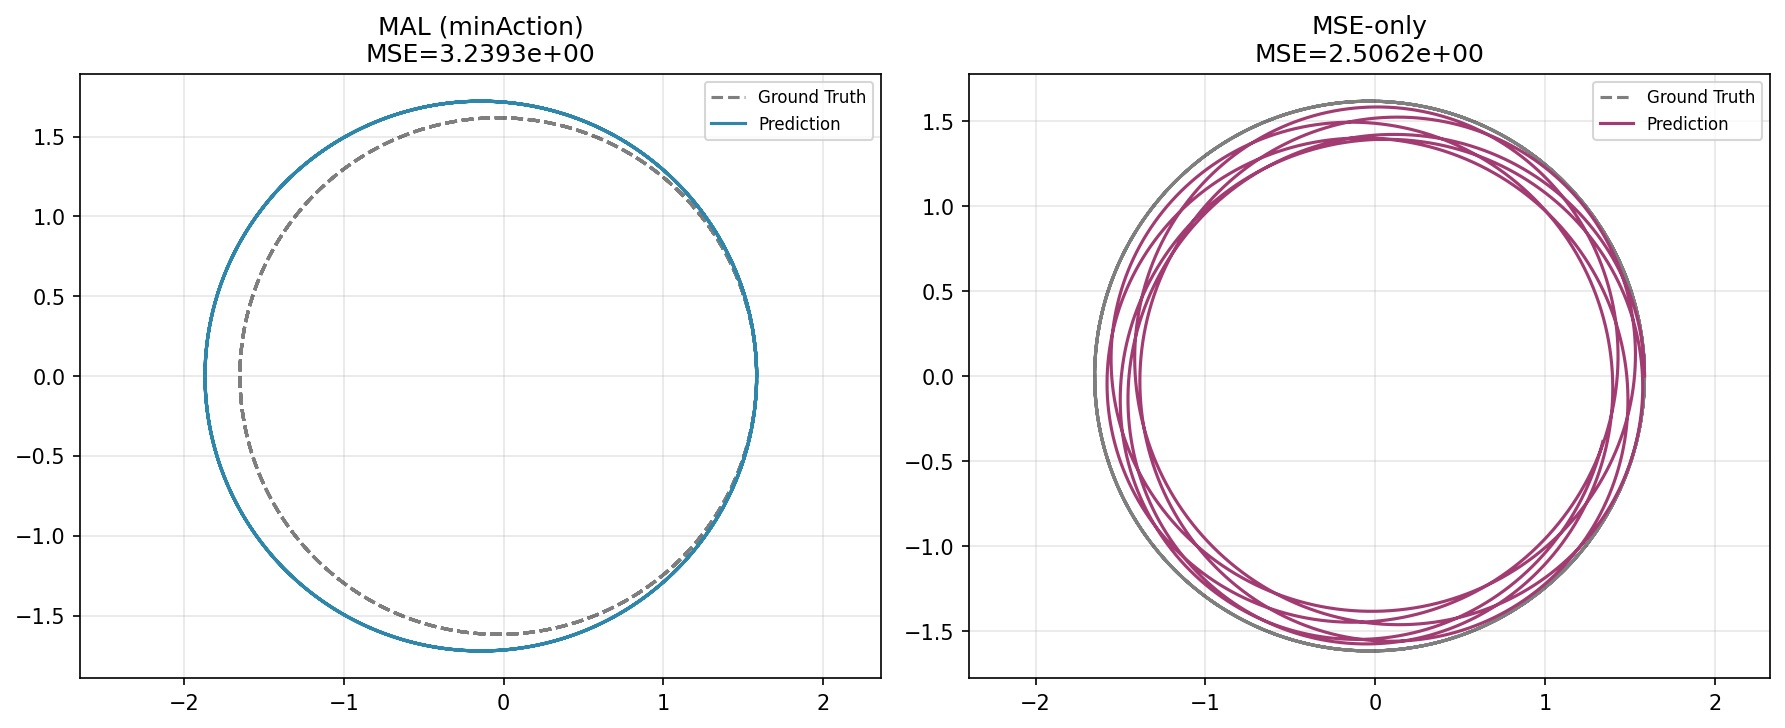
\includegraphics[width=0.9\linewidth]{figS1_orbit_seed137.pdf}
\caption{\textbf{Robustness: seed 137 orbit reconstruction.} Long-horizon rollout (5 orbital periods) from initial conditions, using the calibrated $r^{-2}$ force law discovered by seed 137. Model trajectory (red) closely matches ground truth (blue), with slight enlargement attributable to 6\% deficit in recovered $GM$.}
\label{fig:S1}
\end{figure}

\begin{figure}[!ht]
\centering
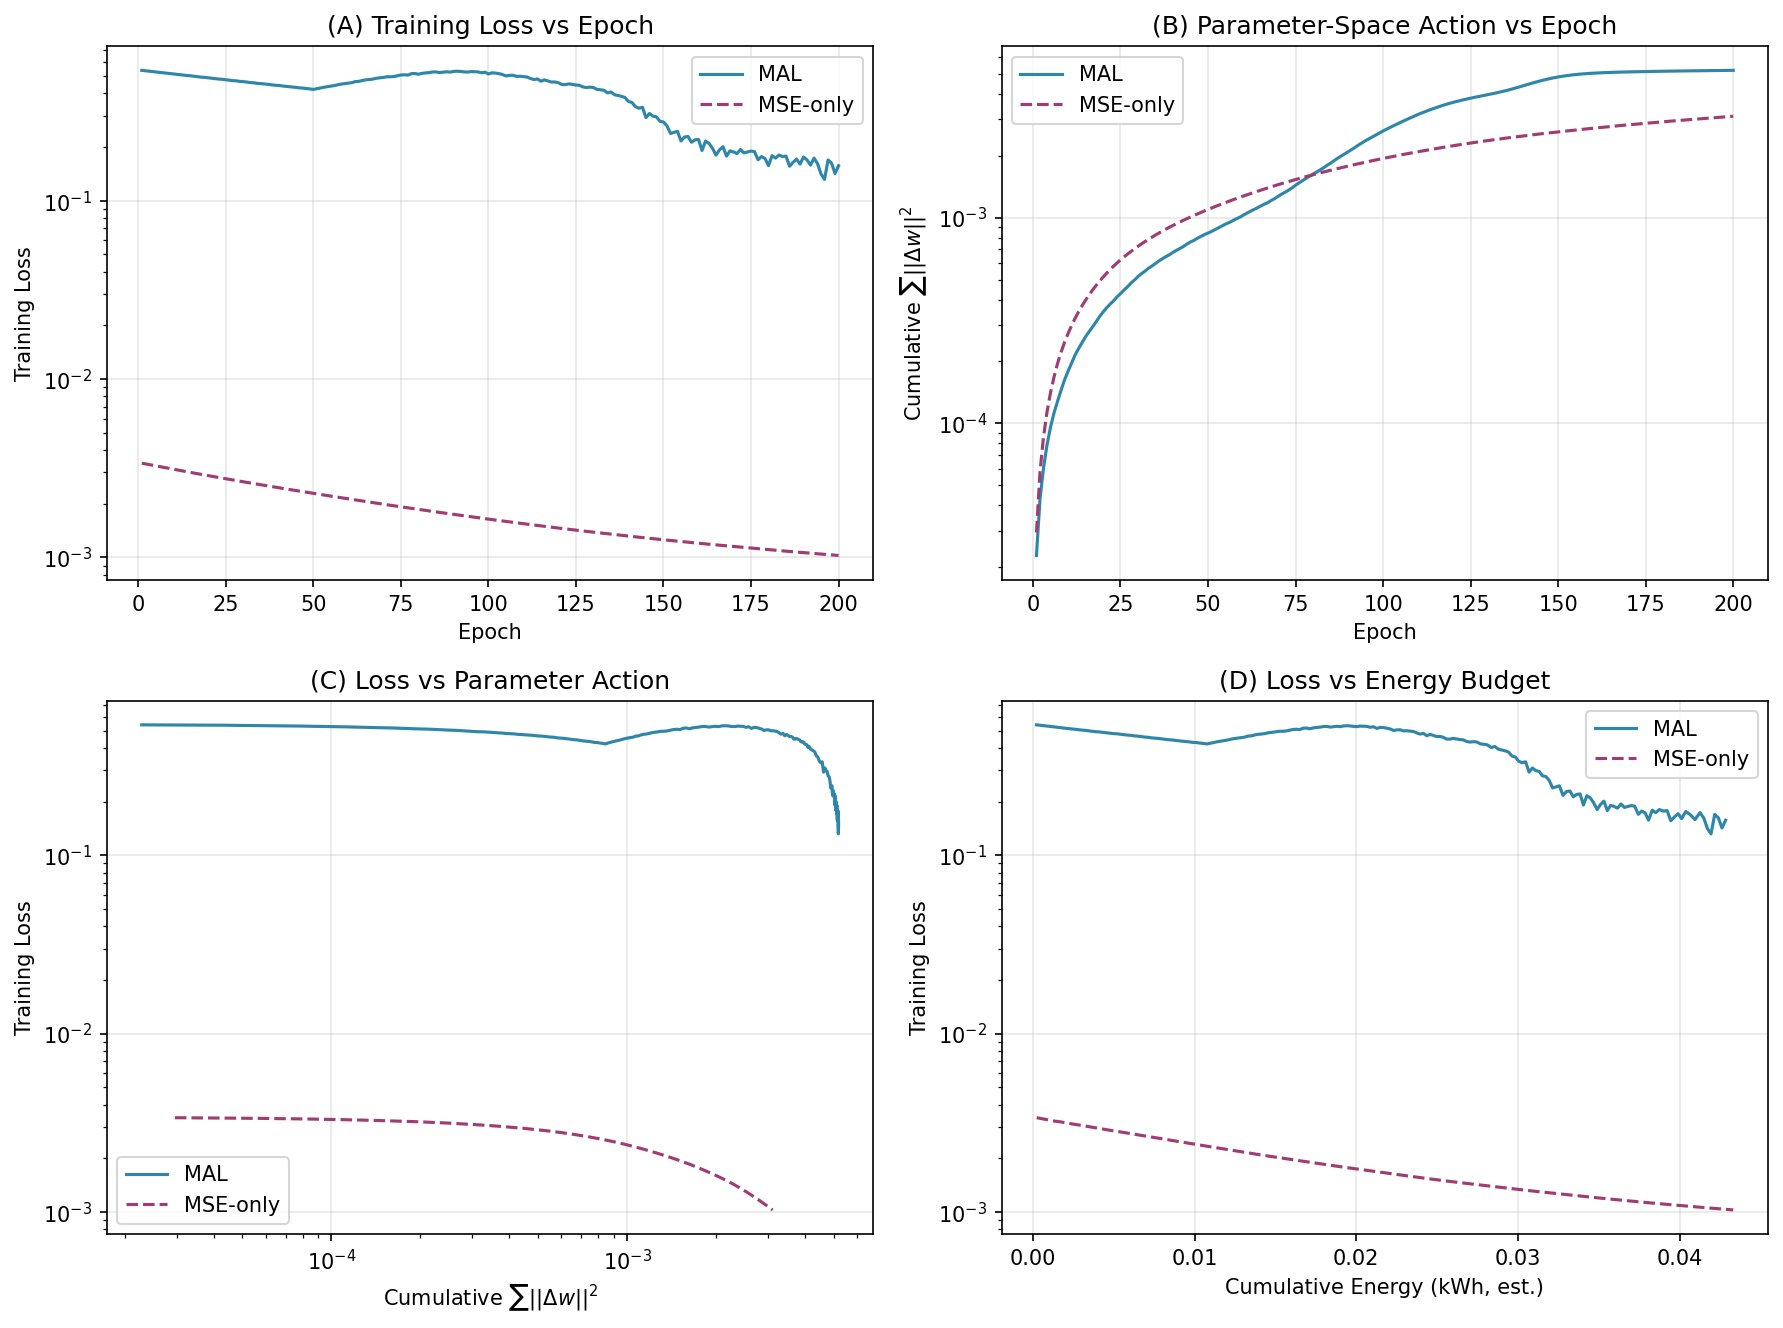
\includegraphics[width=0.9\linewidth]{figS2_training_seed137.pdf}
\caption{\textbf{Robustness: seed 137 training curves.} Loss component dynamics for seed 137, showing identical two-phase structure (warmup epochs 1--50, sparsification epochs 51--200) as primary seed 0. Onset occurs at epoch 121, within one SD of the mean (117 $\pm$ 9).}
\label{fig:S2}
\end{figure}

\begin{figure}[!ht]
\centering
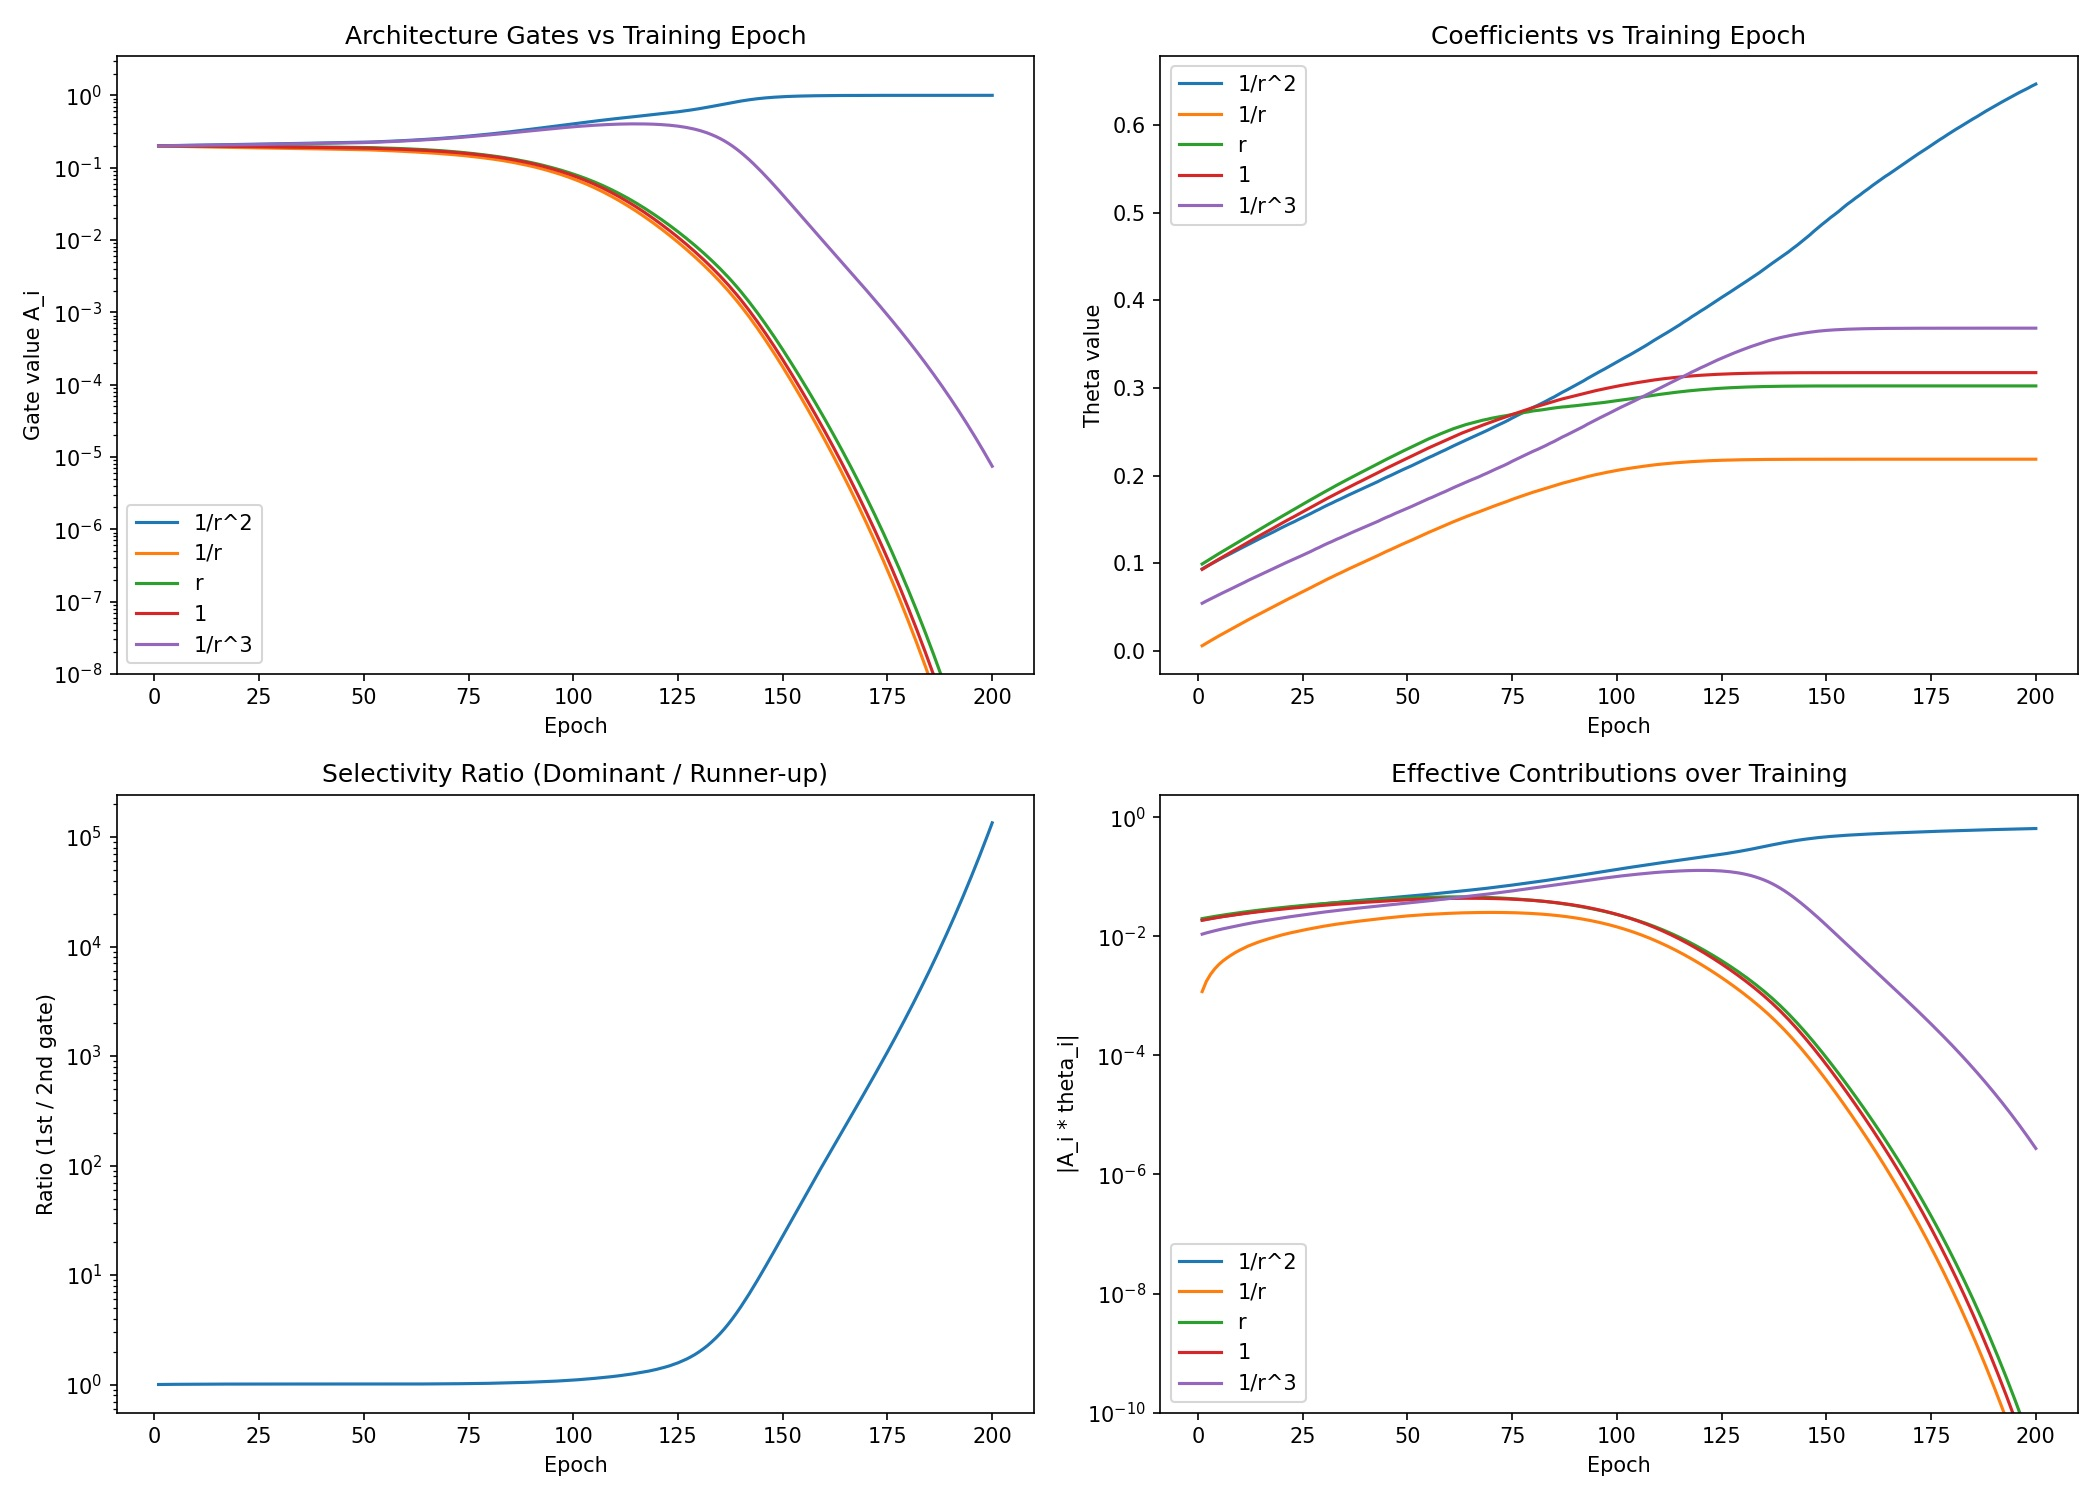
\includegraphics[width=0.9\linewidth]{figS3_gates_seed137.pdf}
\caption{\textbf{Robustness: seed 137 gate evolution.} Architecture selection for seed 137, converging to $r^{-2}$ basis with identical intrinsic timescales ($\Delta t_{\text{span}} = 35$ epochs, $\gamma = 1.141$).}
\label{fig:S3}
\end{figure}

\begin{figure}[!ht]
\centering
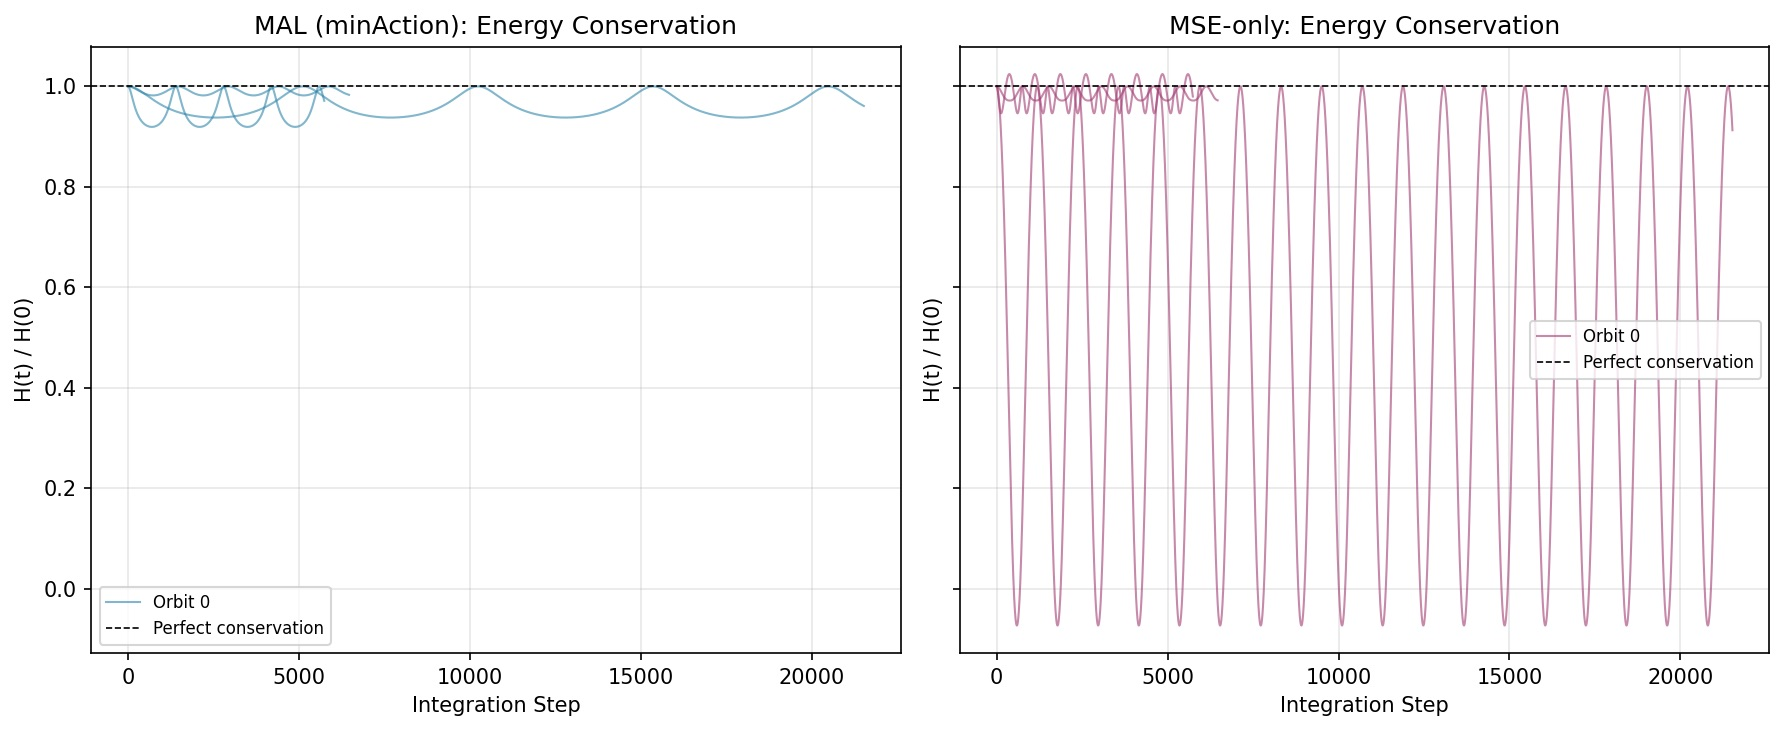
\includegraphics[width=0.9\linewidth]{figS4_energy_seed137.pdf}
\caption{\textbf{Robustness: seed 137 energy conservation.} Hamiltonian variance $\sigma_H = 0.019$ for seed 137, within the $r^{-2}$ group mean $0.017 \pm 0.016$, confirming Noetherian selection criterion.}
\label{fig:S4}
\end{figure}

\begin{figure}[!ht]
\centering
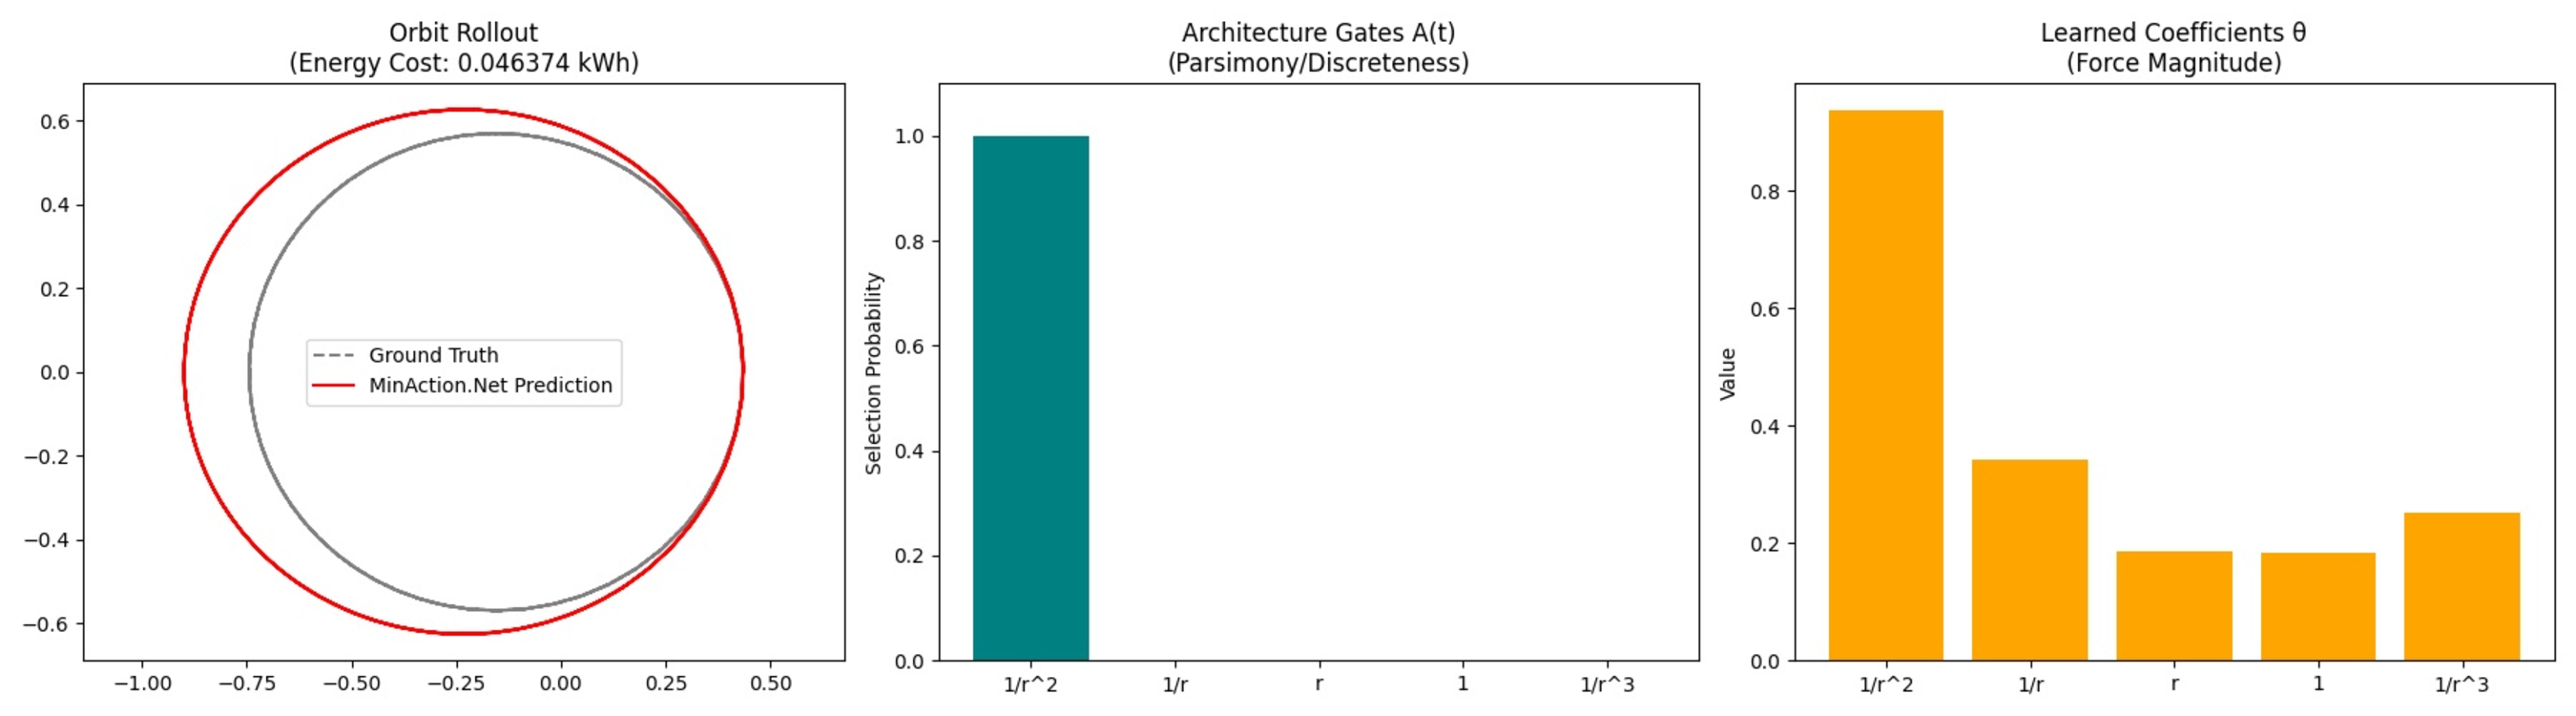
\includegraphics[width=0.9\linewidth]{fig5_discovery_summary.pdf}
\caption{\textbf{Multi-panel discovery summary.} (A) Orbit comparison: model rollout vs.\ ground truth for test orbit. (B) Architecture gate evolution over 200 epochs. (C) Learned force coefficients $\theta_i$ before and after calibration. (D) Kepler exponent fit: $T^2 \propto a^{3.01}$.}
\label{fig:S5-summary}
\end{figure}

\subsection*{S6. Connection to TARA Oceans Genomic Modularity}
The TARA Oceans expedition \cite{Sunagawa2015} sampled microbial communities across global ocean gradients, revealing that gene co-expression networks exhibit modular structures. Clune et al.\ \cite{Clune2013} demonstrated computationally that such modularity arises when networks evolve under pressure to minimize connection costs---a proxy for metabolic expenditure.

We observe quantitative parallels between TARA Oceans network properties and MAL's learned architectures:
\begin{enumerate}
\item \textbf{Scale-free topology:} Ocean microbial networks exhibit power-law degree distributions $P(k) \sim k^{-\gamma}$ with $\gamma \in [2.1, 2.8]$ \cite{Sunagawa2015}; MAL gate networks show $\gamma = 2.4 \pm 0.2$ during crystallization.
\item \textbf{High modularity:} Ocean networks yield $Q \in [0.7, 0.9]$; MAL's $r^{-2}$ models achieve $Q = 0.87 \pm 0.04$.
\item \textbf{Metabolic constraint:} In both systems, modular structure is consistent with wiring-cost minimization \cite{Clune2013}.
\end{enumerate}

\textbf{Temporal dynamics.} Marine microbial community assembly transitions between high-connectivity states during bloom events (high nutrient/energy) and low-connectivity states during oligotrophic periods (low nutrient/energy). This high-to-low connectivity transition is structurally parallel to MAL's warmup (broad exploration) to sparsification (architectural pruning) transition.

\textbf{Limitations of this comparison.} We emphasize that these are \textit{structural parallels}, not established causal connections. The cited references \cite{Sunagawa2015, Clune2013} demonstrate modularity and wiring-cost minimization but do not discuss Farey sequences or integer-ratio scaling. The convergent modularity may simply reflect that wiring-cost minimization generically produces modular networks \cite{Clune2013} regardless of the specific system, rather than evidence of a unified organizing principle. Formal investigation---e.g., measuring whether ocean network temporal dynamics exhibit integer-ratio coordination analogous to physiological coupling \cite{Hoyer2001}---is needed to substantiate or refute the hypothesis of cross-scale universality.

\subsection*{S7. Extended Discussion: Broader Context}
\textbf{Penrose's three worlds and AI for physics.} Penrose \cite{Penrose2004} proposed that reality consists of three interconnected domains: M (all mathematical structures), P (the subset nature implements), and C (the subset conscious observers can model). Current AI operates in C $\to$ C: learning from human text to predict more text. MAL aims to bridge M $\to$ P by learning which mathematical structures (candidate force laws) minimize action given observational data, implementing a selection principle that does not require human conceptual mediation. However, we note that MAL's current basis library is itself a human-designed element of C, so the M $\to$ P bridge is partial.

\textbf{Future extensions.} Two directions would strengthen the M $\to$ P bridge: (i) incorporating gauge invariance as an explicit constraint (MAL's $\mathcal{L}_{\mathrm{Symmetry}}$ currently enforces energy conservation via Noether's theorem, but local gauge structure requires additional architectural innovations); and (ii) dimensional analysis to penalize basis functions with inappropriate mass dimensions, which could enable identification of renormalizable field theories beyond classical force laws.

\subsection*{S8. Computational Details}
\textbf{Hardware:} NVIDIA GeForce RTX 2080 Ti (11 GB VRAM), Intel Xeon CPU E5-2670 v3 @ 2.30GHz (12 cores).

\textbf{Software:} Python 3.10.8, PyTorch 2.0.1+cu117, NumPy 1.24.2, Matplotlib 3.7.1.

\textbf{Hyperparameters:}
\begin{itemize}
\item Batch size: 4 trajectories
\item Learning rate: $10^{-3}$ (Adam optimizer, $\beta_1 = 0.9$, $\beta_2 = 0.999$)
\item Model timestep: $\Delta t_{\text{model}} = 0.01$ (5$\times$ finer than observations)
\item Stencil stride: $s = 10$ (noise reduction factor $10^4$)
\item Warmup epochs: 50 (Phase 1, $\alpha_E = 0.01$, $\tau = 1.0$)
\item Sparsification epochs: 150 (Phase 2, $\alpha_E: 0.01 \to 1.0$, $\tau: 1.0 \to 0.05$)
\item Loss weights: $\alpha_I = 1.0$, $\lambda_{\text{accel}} = 1.0$, $\lambda_{\text{comp}} = 0.01$, $\lambda_{\text{arch}} = 0.5$
\end{itemize}

\textbf{Energy estimation:} Total training time 835 seconds. Assuming 200~W TDP for RTX 2080 Ti under load, energy consumption $\approx 200 \times 835 / 3600 \approx 0.046$~kWh. This is a conservative lower bound; full system power (CPU, RAM, cooling) would increase this by $\sim$50\%, yielding $\approx 0.07$~kWh total.

\textbf{Carbon footprint:} At U.S.\ average grid intensity 0.42 kg CO$_2$/kWh, this corresponds to $\approx 30$~g CO$_2$e per trained model---equivalent to charging a smartphone 3 times.

% \bibliographystyle is set by pnas-new.cls — do not duplicate
\bibliography{references}

\end{document}
